\documentclass[12pt]{article}

\usepackage[margin = 1in]{geometry}
\usepackage{graphicx}              
\usepackage{amsmath}               
\usepackage{amsfonts}              
\usepackage{amsthm}                
\usepackage{amssymb}
\usepackage{mathrsfs}
\usepackage{url}
%\usepackage{subfig}
%\usepackage{xfrac}
%\usepackage[sectionbib]{chapterbib}
\usepackage{hyperref}
\usepackage{tikz}
\usetikzlibrary{positioning,calc,arrows}
\usepackage{algorithmic}
\usepackage{afterpage}
\usepackage{pdflscape}
\usepackage{subcaption}

\hypersetup{
	unicode=true,
	colorlinks=true,
	citecolor=black,
	filecolor=black,
	linkcolor=black,
	urlcolor=black,
	pdfstartview={FitH},
}

% theorem environments
\theoremstyle{plain}
\newtheorem{theorem}{Theorem}
\newtheorem{lemma}[theorem]{Lemma}
\newtheorem{corollary}[theorem]{Corollary}
\newtheorem{proposition}[theorem]{Proposition}
\theoremstyle{definition}
\newtheorem{definition}[theorem]{Definition}
\newtheorem{conjecture}[theorem]{Conjecture}
\newtheorem{example}[theorem]{Example}
\newtheorem*{remark}{Remark}
\newtheorem{note}[theorem]{Note}


\renewcommand{\algorithmicrequire}{\textbf{Input:}}
\renewcommand{\algorithmicensure}{\textbf{Output:}}
\algsetup{linenodelimiter=.}

\newcommand{\wrt}{\vdash} 
\newcommand{\ang}[1]{\langle#1\rangle}
\newcommand{\abs}[1]{\left\vert#1\right\vert}
\newcommand{\dual}[1]{\overline{#1}}
\newcommand{\mapsfrom}{\ensuremath{\reflectbox{$\mapsto$}}}
\newcommand{\tildO}{\tilde{O}}
% roman numerals
\newcommand{\romnum}[1]{\romannumeral #1}
\newcommand{\Romnum}[1]{\uppercase\expandafter{\romannumeral #1}}

\newcommand{\todo}[1]{\textcolor{red}{TODO: #1}}
\newcommand{\comment}[2][Note]{\textcolor{green}{(#1): #2}}

\DeclareMathOperator{\fieldchar}{char} % characteristic of a field
\DeclareMathOperator{\ringofend}{End} % endomorphism ring
\DeclareMathOperator{\trace}{Tr} % finite field trace
\DeclareMathOperator{\gal}{Gal} % Galois group
\DeclareMathOperator{\order}{ord} % order of an element
\DeclareMathOperator{\lcm}{lcm} % least common multiple
\DeclareMathOperator{\divisor}{div} % divisor on a curve
\DeclareMathOperator{\supp}{supp} % support of a divisor
\DeclareMathOperator{\norm}{N} % norm
\DeclareMathOperator{\Res}{Res}
\DeclareMathOperator{\Aut}{Aut}
\DeclareMathOperator{\minpoly}{minpoly}
\DeclareMathOperator{\loglog}{loglog}
\DeclareMathOperator{\rev}{rev}

\def\Q{\ensuremath{\mathbb{Q}}}
\def\N{\ensuremath{\mathbb{N}}}
\def\R{\ensuremath{\mathbb{R}}}
\def\Z{\ensuremath{\mathbb{Z}}}
\def\F{\ensuremath{\mathbb{F}}}
% \def\H{\ensuremath{\mathbb{H}}}
% \def\K{\ensuremath{\mathbb{K}}}
% \def\L{\ensuremath{\mathbb{L}}}
% \def\A{\ensuremath{\mathbb{A}}}
% \def\B{\ensuremath{\mathbb{B}}}
\def\MM{\ensuremath{\mathsf{M}}}
\def\MMM{\ensuremath{\mathsf{MM}}}
% \def\MC{\ensuremath{\mathsf{C}}}
% \def\PC{\ensuremath{\mathsf{PC}}}
% \def\II{\ensuremath{\mathsf{I}}}
% \def\QQ{\ensuremath{\mathsf{Q}}}
\def\CC{\ensuremath{\mathsf{C}}}
% \def\RR{\ensuremath{\mathsf{R}}}
% \def\AA{\ensuremath{\mathsf{A}}}
% \def\va{\ensuremath{\mathsf{a}}}
% \def\vy{\ensuremath{\mathsf{y}}}
% \def\vu{\ensuremath{\mathsf{u}}}
% \def\vb{\ensuremath{\mathsf{b}}}
% \def\vc{\ensuremath{\mathsf{c}}}
% \def\mul{\ensuremath{\mathsf{mul}}}
% \def\rem{\ensuremath{\mathsf{rem}}}
% \def\cat{\ensuremath{\mathsf{cat}}}
% \def\coeff{\ensuremath{\mathsf{coefficient}}}
% \def\mulmod{\ensuremath{\mathsf{mulmod}}}
% \def\x{\ensuremath{\mathbf{x}}}
% \def\uu{\ensuremath{\mathbf{U}}}
% \def\bb{\ensuremath{\mathbf{B}}}
% \def\bxi{\boldsymbol{\xi}}
% \def\bupsilon{\boldsymbol{\upsilon}}
% \def\bzeta{\boldsymbol{\zeta}}
% \def\blambda{\boldsymbol{\lambda}}
\def\euler{\ensuremath{\varphi}}

% allow algorithms to split over multiple pages
\makeatletter
\newcounter{algorithm}
\setcounter{algorithm}{0}
\renewcommand{\thealgorithm}{\arabic{algorithm}}
\def\algorithm{\@ifnextchar[{\@algorithma}{\@algorithmb}}
\def\@algorithma[#1]{%
	\refstepcounter{algorithm}
	\trivlist
	\leftmargin\z@
	\itemindent\z@
	\labelsep\z@
	\item[\parbox{\columnwidth}{%
		\hrule
		\hrule
		\noindent\strut\textbf{Algorithm \thealgorithm} #1
		\hrule
	}]\hfil\vskip0em%
}
\def\@algorithmb{\@algorithma[]}
\def\endalgorithm{\hfil\vskip-1em\hrule\endtrivlist}
\makeatother


\title{Computing isomorphisms and embeddings of finite fields}
\author{Ludovic Brieulle, Luca De Feo, Javad Doliskani,\\ Jean-Pierre
  Flori and \'Eric Schost}


\begin{document}

\maketitle
\begin{abstract}
  Let $\F_q$ be a finite field.  The finite field embedding problem
  asks, given two irreducible polynomials $f,g$ over $\F_q$ with $\deg
  f$ dividing $\deg g$, to compute an explicit description of a field
  embedding of $\F_q[X]/f(X)$ into $\F_q[Y]/g(Y)$. When $\deg f = \deg
  g$, this is also known as the isomorphism problem.
  
  We review classical algorithms for the two problems, and compare
  their asymptotic complexities. We also propose new improvements and
  generalizations to the algorithms, implement them, and compare them
  with the state of the art.
\end{abstract}

\setcounter{tocdepth}{2}
\tableofcontents

%%%%%%%%%%%%%%%%%%%%%%%%%%%%%%%%%%
%%%%%%%%%%%%%%%%%%%%%%%%%%%%%%%%%%

\section*{Proposed notation}

This section is for internal reference only: erase after the paper has
stabilized.

\begin{itemize}
\item Base field: $\F_q$. Characteristic: $p$ (use it as little as
  possible). When algorithms only apply if $p=q$, state explicitly
  (verbally) that $q$ is prime.
\item Quotient notation: $\F_q[X]/f(X)$ or $\F_q[X]/(X^a-b)$, or
  $\F_q[X,Y]/(X^3,Y^6)$.
\item Other fields: $k = \F_q[X]/f(X)$, $K = \F_q[Y]/g(Y)$.
\item $m = \deg f, n=\deg g$, $m|n$.
\item $r$ a prime power dividing $m$.
\item $\phi,\psi$ embeddings.
\item Field trace $\trace$.
\item $\euler$: Euler function.
\item $\Phi_r$ cyclotomic polynomial, also modular polynomial.
\item $h$: factor of the cyclotomic polynomial.
\item Elliptic curves: $E:y^2=x^3+ax+b$ or $E:y^2+a_1xy+a_3y=x^3+\cdots$.
\item $\psi_m$ division polynomial, $\omega$ invariant differential.
\item $\pi$ frobenius endomorphism (elliptic curves), $t$ its trace,
  $\lambda,\mu$ its eigenvalues.
\item $s$ order of $q$ mod $r$ (Kummer), degree of auxiliary extension (Rains).
\item $\ell$ prime (power) such that $r|\order_\ell q$ (Rains).
\item modular integers: $\Z/m\Z$,
\item multiplicative groups: $\F_q^\ast$ and $(\Z/m\Z)^\ast$.
\item $S$ subgroup of Galois group. $\langle s,t \rangle$ subgroup
  generated by $s$ and $t$.
\item $\sigma$ element of Galois group.
\item $\zeta$ root of unity. $\mu_x$ roots group of order $x$.
\item $\eta$, $\eta_a$, $\eta(\zeta)$ periods.
\item $L$ number field, $\mathcal{O}_L$ integer ring.
\item $\alpha,\beta$ outputs of embedding description algorithms.
\item $\gamma,\delta$ inputs/outputs of embedding evaluation algorithms.
\item Complexity: $O$, $\tildO$. $\MM$ polynomial multiplication,
  $\CC$ modcomp, $\MMM(n)$ and $\MMM(m,n)$ matrix multiplication.
\item Free symbols (for use internal to sections):
  $a,b,c,d,e,i,j,t,u,v,w,z$,
  $\varepsilon,\epsilon,\theta,\xi,\kappa,\nu,\rho,\chi,\upsilon,\tau$,
  $A,B,C,D,E,F,G,H,I,J,M,N,Q,R,T,U,V$,
  $\Gamma,\Delta,\Theta,\Lambda,\Xi,\Psi,\Omega$.
\end{itemize}




\section{Introduction}
\label{sec:introduction}

Let $q$ be a prime power and let $\F_q$ be a field with $q$
elements. Let $f$ and $g$ be irreducible polynomials over $\F_q$, with
$\deg f$ dividing $\deg g$. Define $k=\F_q[X]/f(X)$ and
$K=\F_q[Y]/g(Y)$, then there is an embedding $\phi:k\hookrightarrow
K$, unique up to $\F_q$-automorphisms of $k$. The goal of this paper
is to describe algorithms to efficiently represent and evaluate one
such embedding.

\todo{Motivation, previous work.}

All the algorithms we are aware of, split the embedding problem in two
sub-problems:
\begin{enumerate}
\item Determine elements $\alpha\in k$ and $\beta\in K$ such that
  $k=\F_q[\alpha]$, and such that there exists an
  embedding $\phi$ mapping $\alpha\mapsto\beta$. We refer to this
  problem as the \emph{Embedding description}.
  It is easily seen that $\alpha$ and $\beta$ describe an embedding
  if and only if they share the same minimal polynomial.
\item Given elements $\alpha$ and $\beta$ as above, given $\gamma\in
  k$ and $\delta\in K$, solve the following problems:
  \begin{itemize}
  \item Compute $\phi(\gamma)\in K$.
  \item Test if $\delta\in\phi(k)$.
  \item If $\delta\in\phi(k)$, compute $\phi^{-1}(\delta)\in k$.
  \end{itemize}
  We refer collectively to these problems as the \emph{Embedding
    evaluation}.
\end{enumerate}


\paragraph{Fundamental algorithms and complexity}
We review the fundamental building blocks that constitute the
algorithms presented next.  We are going to measure all complexities
in number of operations $+$, $\times$, $\div$ in $\F_q$, unless
explicitly stated otherwise. Most of the algorithms we present are
randomized; we use the \emph{big-Oh} notation $O()$ to express average
asymptotic complexity, and we will make it clear when this complexity
depends on heuristics. We also occasionally use the notation
$\tildO()$ to neglect logarithmic factors in the parameters.

We let $\MM(m)$ be a function such that polynomials in $\F_q[X]$ of
degree less than $m$ can be multiplied in $\MM(m)$ operations in
$\F_q$, under the assumptions of~\cite[Ch.~8.3]{vzGG}. Using FFT
multiplication, one can take $\MM(m)\in O(m\log (m) \loglog (m))$.

We denote by $\omega$ the \emph{exponent of linear algebra}, i.e.\ a
constant such that $m\times m$ matrices with coefficients in any field
$k$ can be multiplied using $O(m^\omega)$ additions and
multiplications in $k$.

Some algorithms will operate in a polynomial ring $k[Z]$, where $k$ is
a field extension of $\F_q$. Some other algorithms will operate in
$k[Z]/h(Z)$, where $h$ is a monic polynomial in $k[Z]$. We review the
basic operations in these rings. We assume that $k$ is represented as
a quotient ring $\F_q[X]/f(X)$, with $m=\deg f$, and we let $s=\deg h$
in the complexity estimates.

Multiplying and dividing polynomials of degree at most $s$ in $k[Z]$
is done in $O(\MM(sm))$ operations in $\F_q$, using Kronecker's
substitution~\cite{moenck76,kaltofen87,vzGG,vzgathen+shoup92,harvey09}.
Multiplication in $k[Z]/h(Z)$ is also done in $O(\MM(sm))$ using the
technique in~\cite{pascal+schost06}. By the same techniques, gcds in
$k[Z]$ and inverses in $k[Z]/h(Z)$ are computed in $O(\MM(sm)\log(sm))$.

Given polynomials $e,g,h,\in k[Z]$ of degree at most $s$, modular
composition is the problem of computing $e(g) \bmod h$. An upper bound
on the algebraic complexity of modular composition is obtained by the
Brent-Kung algorithm~\cite{brent+kung}, which takes
$O(s^{1/2}\MM(sm) + s^{(\omega+1)/2}\MM(m))$ operations in $\F_q$.  In
the binary RAM complexity model, the Kedlaya-Umans
algorithm~\cite{KeUm11} and its extension in~\cite{PoSc13a} yield an
algorithm with essentially linear complexity in $s$, $m$ and
$\log(q)$. Unfortunately, making these algorithms competitive in
practice is challenging; we are not aware of any implementation of
them. Hence, we will restrict to an algebraic complexity model, denote
by $\CC(s,m)$ the complexity of modular composition in $k[Z]$, and use
$O(s^{1/2}\MM(sm) + s^{(\omega+1)/2}\MM(m))$ as an upper bound.  We
will use $\CC(s)$ as a shorthand notation for $\CC(s,1)$.


\paragraph{Computing subfields.}
With $k = \F_q[X]/f(X)$ and $\deg f=m$ as above, we are given a
divisor $r$ of $m$, and we want to construct an intermediate extension
$\F_q \subset L \subset k$ of degree $r$ over $\F_q$. More precisely,
we want to compute a monic irreducible polynomial $g \in \F_q[X]$ of
degree $r$, and a polynomial $h \in \F_q[X]$ such that
$x \mapsto h(x)\bmod f$ defines an embedding
$L = \F_q[X] / g(X) \hookrightarrow k$. We proceed as follows.

Let $\alpha\in k$ be a random element not in $\F_q$. Then $\alpha$ has a minimal polynomial of degree $m$ 
over $\F_q$ with high probability. In other words, one needs $O(1)$ such random elements to find 
one with degree $m$ minimal polynomial. Now, the trace
\begin{equation}
	\label{equ:trace-simple}
	\trace_{k/L}(\alpha) = \alpha + \alpha^{q^r} + \cdots + \alpha^{q^{m - r}}
\end{equation}
has a minimal polynomial of degree $r$ over $\F_q$ with high
probability as well. This means we can compute, after $O(1)$ random
trials, the desired polynomials $\beta = \trace_{k/L}(\alpha)$,
$g = \minpoly(\beta)$, and $h$ the polynomial of degree $<m$ representing $\beta$.

\begin{proposition}
	\label{prop:subfield}
	Let $\F_q \subset k$ be a finite extension of degree $m$, and
        let $r$ be a divisor of $m$.  Computing an intermediate field
        $\F_q \subset L \subset k$ with $[L:\F_q]=r$ takes
        $O(\CC(m)\log(m) + \MM(m)\log(q))$ operations in $\F_q$.  Once
        $L$ is computed, any element $\gamma\in L$ can be lifted to
        its image in $k$ using $C(m)$ operations.
\end{proposition}
\begin{proof}
	Computing the minimal polynomial of an element in $k$ takes $O(\CC(m))$ operations in $\F_q$, 
	see \cite{shoup93}. It remains to compute the trace in Eq.~\eqref{equ:trace-simple}. This can be done 
	recursively as follows. Let $x$ be the image of $X$ in $k$,
        let $\xi_i = x^{q^{ir}}$, and let $T_i(\alpha) = \alpha + \alpha^{q^r} + \cdots + \alpha^{q^{(i - 1)r}}$. Then
	\[
	\xi_j = 
	\begin{cases}
	\xi_{j / 2}^{q^{j / 2}} & j \text{ even} \\
	\xi_{j - 1}^q & j \text{ odd}
	\end{cases}, \quad
	T_j(\alpha) = 
	\begin{cases}
	T_{j / 2}(\alpha) + T_{j / 2}(\alpha)^{q^{jr/2}} & j \text{ even} \\
	\alpha + T_{j - 1}(\alpha)^{q^r} & j \text{ odd}
	\end{cases}
	\]
	Raising an element $\beta \in k$ to the power of $q^j$ is the same computing the composition 
	$\beta(\xi_j)$. This means that each step of the above recursion is done using $O(1)$ modular 
	compositions in $k$. The depth of the recursion is $\log(i)$. Therefore, given the initial value 
	$\xi_1$, $T_i(a)$ is computed using $O(\CC(m)\log(i))$ operations in $\F_q$. To compute the 
	initial value $\xi_1 = x^{q^r}$ we first compute $x^q$ using the usual binary-powering 
	algorithm at a cost of $O(\MM(m)\log(q))$ operations in $\F_q$. Then the rest is done using the 
	same recursive technique as above at the cost of $O(\CC(m)\log(r))$ operations in $\F_q$. 
	Therefore, computing the trace $\trace_{k/L}(\alpha) = T_{m/r}(\alpha)$ takes $O(\CC(m)\log(m) + 
	\MM(m)\log(q))$ operations in $\F_q$.

        Finally, given an element $\gamma\in L$, its image in $k$ is
        computed by evaluating $h(\gamma)$, where $h$ is the
        polynomial representation of $\trace_{k/L}(\alpha)$. This can
        be done by a modular composition at cost $\CC(m)$.
\end{proof}


\paragraph{Polynomial factorization}
Finally, given a field $k = \F_q[X]/f(X)$ of degree $m$ as above, we will need to
factor some special polynomials in $k[Z]$. More precisely, we are
interested in finding one factor of a polynomial that splits into
factors of the same, known, degree. This problem is known as
\emph{equal degree factorization} (EDF), and the best generic algorithm for
it is the Cantor-Zassenhaus method~\cite{cantor1981,von1992computing},
which runs in $O(\MM(sm)(dm\log(q) + \log(sm)))$ operations in
$\F_q$~\cite[Th.~14.9]{vzGG}, where $s$ is the degree of the
polynomial to factor, and $d$ is the degree of the factors.

More efficient variants of the Cantor-Zassenhaus method are known for
special cases. When the degree $s$ of the polynomial is small compared
to the extension degree $m$, Kaltofen and Shoup~\cite{kaltofen+shoup97} 
give an efficient algorithm which is as follows.

\begin{algorithm}[Kaltofen-Shoup EDF for extension fields]
	\label{alg:ks}
	\begin{algorithmic}[1]
		\REQUIRE A polynomial $h$ of degree $s$ with irreducible factors of degree $d$ over $k$.
		\ENSURE An irreducible factor of $h$ over $k$.
		\STATE If $\deg h = d$ return $h$.
		\STATE Take a random polynomial $a_0\in k[Z]$ of degree less than $s$,
		\STATE\label{alg:ks-pseudotrace} Compute $\displaystyle a_1 
		\leftarrow \sum_{i=0}^{[k:\F_q]d-1} a_0^{q^i} \mod h$,
		\IF{$q$ is an even power $q=2^e$}
		\STATE\label{alg:ks:even} Compute $\displaystyle a_2 \leftarrow 
		\sum_{i=0}^{e-1} a_1^{2^i}\mod h$
		\ELSE
		\STATE\label{alg:ks:odd} Compute $a_2 \leftarrow a_1^{(q-1)/2}\mod h$
		\ENDIF
		\STATE\label{alg:ks:gcd} Compute $h_0\leftarrow\gcd(a_2,h)$ and 
		$h_1\leftarrow\gcd(a_2-1,h)$ and $h_{-1}\leftarrow h/(h_0h_1)$,
		\STATE Apply recursively to the smallest non-constant polynomial among 
		$h_0,h_1,h_{-1}$.
	\end{algorithmic}
\end{algorithm}

We address the reader to the original paper~\cite{kaltofen+shoup97}
for the correctness of the Kaltofen-Shoup algorithm. We redo the
complexity analysis below, to adapt to our framework.

\begin{proposition}
  Given $h$ and $f$ of degrees $s$ and $m$ respectively, the
  Kaltofen-Shoup algorithm finds a factor of $h$ of degree $d$ in
  $k=\F_q[X]/f(X)$ using
  $O\bigl((s\CC(m) + \CC(s,m) + \MM(sm)\log q)\log(dm)\bigr)$
  operations in $\F_q$.
\end{proposition}
\begin{proof}
	It is evident that the dominating step in the Kaltofen-Shoup
	algorithm is the computation of the trace-like function at
	Step~\ref{alg:ks-pseudotrace}. By using a divide-and-conquer
	strategy, they show in~\cite{kaltofen+shoup97} how to compute it in
	$\log (dm)$ steps, using at each step
	\begin{itemize}
		\item $O(s)$ modular compositions in $\F_q[X]$,
		\item $O(1)$ modular compositions in $k[Z]$,
		\item $\log q$ multiplications in $k[Z]/h(Z)$,
	\end{itemize}
	for a total of
        $O\bigl((s\CC(m) + \CC(s,m) + \MM(sm)\log q)\log(dm)\bigr)$
        operations in $\F_q$.  All other steps are easily seen to be
        within this complexity.
	
	Now we need to estimate the average number of recursive calls. The
	probability that only one of $h_0$, $h_1$ and $h_{-1}$ is
	non-constant is at least $1/2^{s/d-1}$, thus we expect that after
	$O(1)$ attempts the algorithm calls itself on a polynomial of
	smaller degree. When the degree decreases, it decreases by at least
	a half, thus the overall complexity is dominated by the first call.
\end{proof}

Now, we use Algorithm \ref{alg:ks} as our base algorithm to derive some
special cases of polynomial factoring which we will use in subsequent sections.
As the first special case, we consider factoring cyclotomic polynomials


\begin{proposition}
  \label{prop:cyclo}
  Given the $s$-th cyclotomic polynomial $\Phi_s$ and a polynomial $f$ of degree $m$,
  an irreducible factor of $\Phi_s$ of degree $d$ over $k=\F_q[X]/f(X)$ 
  can be computed using $O(sm(\log(d)+\log(m))\log(s) + \MM(sm)\log(sm) + 
  \MM(sm)\log(q))$ operations in $\F_q$.
\end{proposition}
\begin{proof}
  We use Algorithm~\ref{alg:ks} and the optimization techniques given
  in~\cite{shoup94}. We start by analyzing the complexity of a single
  recursive call, using the same notation as in
  Algorithm~\ref{alg:ks}.

  Since we have $Z^s = 1\bmod h(Z)$, the trace-like function in
  Step~\ref{alg:ks-pseudotrace} can be computed modulo $Z^s - 1$. As
  remarked by Shoup~\cite{shoup94}, powerings of the form
  $a\mapsto a^{q^j} \bmod Z^s-1$ boil down to simple permutations of
  the coefficients, which are done using $O(sm)$ operations. After
  computing the trace modulo $Z^s - 1$ we have to reduce it modulo $h$
  which is done by a division with remainder using $O(\MM(sm))$
  operations.  Thus, the total cost for Step~\ref{alg:ks-pseudotrace}
  is $O(\MM(sm) + sm(\log(d)+\log(m)))$.

  If we let $t=\deg h$, the exponentiations in Steps~\ref{alg:ks:even}
  and~\ref{alg:ks:odd} are done in $O(\MM(tm)\log(q))$
  operations. Finally, the gcds in Step~\ref{alg:ks:gcd} are computed
  in $O(\MM(tm)\log(tm))$.

  As analyzed by Shoup, the number of recursive calls is in
  $O(\log(s))$, and at each recursive step the degree of $h$ is halved
  with probability at least $1/2$. Hence, we shall multiply the
  complexity of Step~\ref{alg:ks-pseudotrace} by
  $\log s$, while the first call to Steps~\ref{alg:ks:even},~\ref{alg:ks:odd}
  and~\ref{alg:ks:gcd} dominates all others. Thus the total cost of the algorithm is
  $O(sm(\log(d)+\log(m))\log(s) + \MM(sm)\log(sm) + \MM(sm)\log(q))$.
\end{proof}

As the next special case of Algorithm \ref{alg:ks}, we consider taking roots in cyclotomic
extensions. Let $r$ be a prime power and let $h$ be an irreducible factor of the $r$-th
cyclotomic polynomial $\Phi_r$, with $s = \deg h$. Denote $\F_q[Z] / h(Z)$ by $\F_q(\zeta)$, where 
$\zeta$ is the image of $Z$ in the quotient. Given an $r$-th power $\alpha \in \F_q(\zeta)$ we want 
to compute an $r$-th root $\alpha^{1 / r}$, or equivalently a linear factor of $X^r - \alpha$ over 
$\F_q(\zeta)$.
\begin{proposition}
	\label{prop:root-fpz}
	Let $r$ be a prime power and let $\zeta$ be a primitive $r$-th root of unity. Also let $s = 
	[\F_q(\zeta): \F_q]$. If $s \in O(r^{(3 - \omega) / 2})$ one can take $r$-th roots in 
	$\F_q(\zeta)$ using $O(\MM(s)\log(q)\log(r) + r\CC(s)\log(s) + \MM(rs)\log(s)\log(r))$ 
	operations in $\F_q$. Otherwise, taking $r$-th roots in $\F_q(\zeta)$ can be done in 
	$O(\MM(s)\log(q)\log(r) + r\MM(r)\log(s) + \MM(rs)\log(s)\log(r))$ operations in $\F_q$. 
\end{proposition}
\begin{remark}
	\label{terms-l-s}
	Considering $\CC(r) \in O(r^{(\omega + 1) / 2})$, the condition $s \in O(r^{(3 - \omega) / 
	2})$ is proposed to keep the term $s\CC(r)$, which appears in complexity estimations of 
	subsequent sections, at most quadratic in $r$. This also forces the term $r\CC(s)$ in 
	Proposition \ref{prop:root-fpz} to be subquadratic, hence keeping the complexity in both cases 
	at most quadratic. 
\end{remark}
\begin{proof}
We adapt Algorithm~\ref{alg:ks} to get a linear factor of the polynomial $X^r-\alpha$. 
Again, we discuss Step~\ref{alg:ks-pseudotrace}, which is the dominant 
step. Let $h$ be a factor of $X^r-\alpha$ of degree $n$, and let $x$ be the image of $X$ modulo 
$h$. For clarity, we rewrite the recursion relations in \cite{kaltofen+shoup97}. Let
\[ \beta_i = a_0^q + a_0^{q^2} + \cdots + a_0^{q^i}, \quad \xi_i = x^{q^i}, \quad \zeta_i = \zeta^{q^i}. \]
Then we have $\beta_1 = h^q$, $\xi_1 = x^q$, $\zeta_1 = \zeta^q$, and
\[
\beta_j = 
\begin{cases}
\beta_{j / 2} + \beta_{j / 2}^{q^{j / 2}} & j \text{ even} \\
\beta_1 + \beta_{j - 1}^q & j \text{ odd}
\end{cases}, \quad
\xi_j = 
\begin{cases}
\xi_{j / 2}^{q^{j / 2}} & j \text{ even} \\
\xi_{j - 1}^q & j \text{ odd}
\end{cases}, \quad
\zeta_j = 
\begin{cases}
\zeta_{j / 2}^{q^{j / 2}} & j \text{ even} \\
\zeta_{j - 1}^q & j \text{ odd}
\end{cases}
\]
For a positive integer $j$ we have
\begin{equation}
\label{equation:betaj}
\beta_j^{q^j} = \left( \sum_{\ell = 0}^{n - 1}c_\ell(\zeta)x^\ell \right)^{q^j} = \sum_{\ell = 0}^{n - 
	1}c_\ell(\zeta^{q^j})(x^{q^j})^\ell = \sum_{\ell = 0}^{n - 1}c_\ell(\zeta_j)\xi_j^\ell.
\end{equation}
Now we analyze the running of computing $a_1 = a_0 + \beta_{s - 1}$. First note that we always 
have $\zeta^r = 1, x^r = a$. This makes it possible to keep the identities simple and do the reductions 
at the end of each step. For example $x^q = a^{\lfloor q / r\rfloor}x^{q \bmod r}$ which can be 
computed using $O(\MM(s)\log(q))$ operations in $\F_q$. At step $j$ of the recursion we have the 
following costs in $\F_q$:
\begin{itemize}
	\item $O(\MM(r) + \MM(s)\log(r))$ for computing $x^{q^j}$.
	\item If $s \in O(r^{(3 - \omega) / 2})$ we can first compute $\zeta^{q^j \bmod r}$ modulo $h$, 
	and then do $n$ modular compositions at a total cost of $O(\MM(r) + n\CC(s))$. Otherwise, we  
	reduce $c_\ell(Z^{q^j \bmod r})$ modulo $g(Z)$ for all $0 \le \ell < n$ at a total cost of 
	$O(n\MM(r))$.
	\item $O(n\MM(s))$ for evaluating $\beta_j$ at $x^{q^j}$ using Horner's method.
	\item $O(\MM(rs))$ for reducing (\ref{equation:betaj}) modulo $f$.
\end{itemize}
The depth of the recursion is $\log(s)$, hence $a_1$ can be computed in $O(\MM(s)\log(q) + 
n\CC(s)\log(s) + \MM(rs)\log(s))$ operations in $\F_q$ if $s \in O(r^{(3 - \omega) / 2})$, or
$O(\MM(s)\log(q) + n\MM(r)\log(s) + \MM(rs)\log(s))$ operations in $\F_q$ otherwise. Finally, since 
the depth of the recursion in Algorithm \ref{alg:ks} is $\log(r)$, and the coefficient $n$ is 
halved each time, we have the desired result.
\end{proof}








%%%%%%%%%%%%%%%%%%%%%%%%%%%%%%%%%%
%%%%%%%%%%%%%%%%%%%%%%%%%%%%%%%%%%

\part{Embedding description}

This part is devoted to the problem of describing the embedding of
$k=\F_q[X]/f(X)$ in $K=\F_q[Y]/g(Y)$; we let $m=\deg f$ and
$n=\deg g$, so that $m|n$. The \emph{embedding description problem}
asks to find two elements $\alpha\in k$ and $\beta\in K$ such that
$\alpha\mapsto\beta$ for some field embedding $\phi:k\to K$. This is
equivalent to $\alpha$ and $\beta$ having the same minimal polynomial.

The most obvious way to solve this problem is to take the class of $X$
in $k=\F_q[X]/f(X)$ for $\alpha$, and a root of $f$ in $K$ for
$\beta$. Since $f$ splits completely in $K$, we can apply Algorithm
\ref{alg:ks} for the special case $d = 1$, which gives an upper bound
of $O\bigl((n\CC(m) + \CC(n,m) + \MM(nm)\log q)\log(m)\bigr)$ for the
problem. We remark that this complexity is strictly larger than
$\tildO(m^2)$.

For a more specialized approach, we note that it is enough to solve
the following problem: let $r$ be a prime power such that $r|m$ and
$\gcd(r,m/r)=1$, find $\alpha_r\in k$ and $\beta_r\in K$ such that
$\minpoly(\alpha_r)=\minpoly(\beta_r)$ and $\deg\minpoly(\alpha_r)=r$.

Indeed, once such $\alpha_r$ and $\beta_r$ are known for every primary
factor $r$ of $m$, possible solutions to the embedding problem are
\begin{equation*}
  \alpha = \prod_{\substack{r|m,\\\gcd(r,m/r)=1}}\alpha_r,\qquad
  \beta = \prod_{\substack{r|m,\\\gcd(r,m/r)=1}}\beta_r,
\end{equation*}
or
\begin{equation*}
  \alpha = \sum_{\substack{r|m,\\\gcd(r,m/r)=1}}\alpha_r,\qquad
  \beta = \sum_{\substack{r|m,\\\gcd(r,m/r)=1}}\beta_r.
\end{equation*}

In the next sections, we present algorithms to solve this problem. To
simplify the exposition, we will assume that $[k:\F_q]=[K:\F_q]=r$.
Indeed, we can reduce to this situation by applying
Proposition~\ref{prop:subfield}, at an additional cost of
$O(\CC(n)\log(n) + \MM(n)\log(q))$ for each primary factor $r$.

All algorithms presented next are going to rely on one common
principle: construct an element in $k$ (and in $K$) such that its
minimal polynomial (or, equivalently, its orbit under the absolute
Galois group of $\F_q$) is uniquely (or \emph{almost} uniquely)
defined.






\section{Kummer-type algorithms}
\label{sec:kummer}

In this section we review what we call \textit{Kummer-type} approaches to the embedding problem. 
We briefly review the works of Lenstra \cite{LenstraJr91}, and Allombert \cite{Allombert02}, then 
we give a variant of these algorithms with a significantly lower running time complexity. By 
applying the subfield technique, introduced in Section \ref{sec:introduction}, we assume the 
following reduced version of the embedding problem in the entire section: given extensions $k, K$  
of the same degree $r$ where $r$ is a prime power, construct an embedding $k \hookrightarrow K$. We 
give our fast versions of the algorithms for two separate cases: the case $p \nmid r$, where $p$ is 
the characteristic, is treated in Section \ref{sec:fast-kummer}, and the case $r = p^d$, where $d$ 
is a positive integer, is treated in Section \ref{sec:fast-artin-schreier}.

Let $k$ be an extension of degree $r$ of $\F_q$. In \cite{LenstraJr91}, Lenstra proves that 
given two finite fields of the same size, there exists a deterministic polynomial time algorithm 
that finds an isomorphism between them. The focus of the paper is on the theoretical construction 
of the isomorphism, and no precise complexity analysis is presented. However, since there is an 
explicit assumption of using linear algebra in the paper, a rough analysis of the algorithm yields 
an estimate of $O(r^{\omega})$ operations in $\F_q$. The idea of the algorithm is as follows.

Let $\F_q[\zeta]$ denote the ring extension $\F_q[X] / \Phi_r(X)$ where $\Phi_r$ is the $r$th 
cyclotomic polynomial, and let $\F_q[\zeta][c^{1/r}]$ denote the quotient $\F_q[\zeta][Y]/(Y^r - 
c)$ such that $c^{1/r}$ is the residue class of $Y$. Then we can find $c_1, c_2 \in \F_q[\zeta]$, 
and an integer $j > 0$ such that
\[
\begin{array}{lrll}
\psi: & \F_q[\zeta][c_1^{1/r}] & \rightarrow & \F_q[\zeta][c_2^{1/r}] \\
& c_1^{1/r} & \mapsto & (c_2^{1/r})^j
\end{array}
\]
is an isomorphism. Next, we construct a chain	
\begin{equation*}
	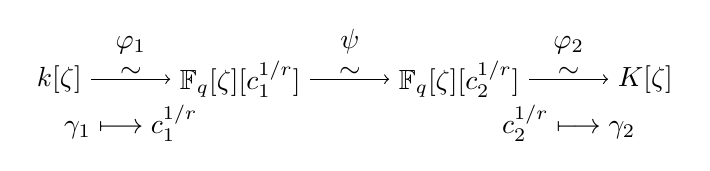
\begin{tikzpicture}
		\node (Fc1) {$\F_q[\zeta][c_1^{1/r}]$};
		\node[right = of Fc1] (Fc2) {$\F_q[\zeta][c_2^{1/r}]$};
		\node[left = of Fc1] (F1) {$k[\zeta]$};
		\node[right = of Fc2] (F2) {$K[\zeta]$};
		\draw[->] (F1) edge node[above, inner sep=0.5pt] {$\sim$} node[above = 3mm, inner 
		sep=0.5pt] {$\varphi_1$} node[below = 3mm, inner sep=0.5pt] {$\gamma_1 \longmapsto 
			c_1^{1/r}$} (Fc1);
		\draw[->] (Fc1) edge node[above, inner sep=0.5pt] {$\sim$} node[above = 3mm, inner 
		sep=0.5pt] {$ \psi $} (Fc2);
		\draw[->] (Fc2) edge node[above, inner sep=0.5pt] {$\sim$} node[above = 3mm, inner 
		sep=0.5pt] {$ \varphi_2 $} node[below = 3mm, inner sep=0.5pt] {$c_2^{1/r} \longmapsto 
			\gamma_2$} (F2);
	\end{tikzpicture}
\end{equation*}
for appropriate $\gamma_1 \in k[\zeta]$, and $\gamma_2 \in K[\zeta]$, and 
homomorphisms $\varphi_1, \varphi_2$. From this we induce an embedding $k \hookrightarrow K$.

In \cite{Allombert02} Alombert gives a similar approach with more focus on implementation. The  
algorithm revolves around solving Hilbert's theorem 90. The idea is to find elements $\alpha_1 \in 
k[\zeta]$, and $\alpha_2 \in K[\zeta]$ such that $b = \alpha_1^r / \alpha_2^r$ is an 
$r$th power in $\F_q[\zeta]$. From this $b^{1/r}$ can be computed using a root extraction 
algorithm. An isomorphism $k[\zeta] \xrightarrow{\sim} K[\zeta]$ is then given by $\alpha_1 
\mapsto b^{1/r}\alpha_2$. Although again no rigorous complexity analysis is presented, one can 
easily see that the dominant cost of this algorithm is solving Hilbert 90 which is done using 
linear algebra. Therefore, the algorithm runs in $O(r^{\omega})$ operations in $\F_q$. We will give 
a more detailed description of the algorithm in the next section.


\subsection{Fast Kummer algorithm for $p \nmid r$}
\label{sec:fast-kummer}

In this section, we present a fast variant of Allombert's algorithm using an explicit solution to 
the Hilbert's theorem 90. Let $[k: \F_q] = r$ where $r$ is a prime power. Let $h(Z)$ be an 
irreducible factor of the $r$-th cyclotomic polynomial over $\F_q$. Then $h$ has degree $s$ where 
$s$ is the order of $q$ in the multiplicative group $\Z/r\Z$. We form the field extension 
$\F_q(\zeta) \cong \F_q[Z] / h$ and the ring extension $k[\zeta] \cong k[Z] / h \cong k \otimes 
\F_q(\zeta)$ where $\zeta$ is the image of $Z$ in the quotients \todo{$k[\zeta]$ is typically used for the FIELD obtained by adjoining $\zeta$ to $k$, this notation is confusing}. The action of the Galois group 
$\gal(k / \F_q)$ can be extended to $k[\zeta]$ by
\[
\begin{array}{llll}
\sigma: & k[\zeta] & \rightarrow & k[\zeta] \\
& x \otimes \zeta & \mapsto & x^q \otimes \zeta.
\end{array}
\]
Then the fixed field of $\sigma$ is $\F_q(\zeta)$. The same can be done for the ring $K[\zeta]$. 
Let us restate the algorithm for clarity.

\begin{algorithm}[Allombert]
	\begin{algorithmic}[1]
		\REQUIRE field extensions $k, K$ of $\F_q$ of degree $r$
		\ENSURE an isomorphism $k \xrightarrow{\sim} K$
		\STATE factor the $r$th cyclotomic polynomial and make the extensions $\F_q(\zeta), 
		k[\zeta], K[\zeta]$
		\STATE find $\theta_1 \in k[\zeta]$ such that $\sigma(\theta_1) = \zeta\theta_1$
		\STATE find $\theta_2 \in K[\zeta]$ such that $\sigma(\theta_2) = \zeta\theta_2$
		\STATE compute an $r$th root $c$ of $\theta_1^r / \theta_2^r$ in $\F_q(\zeta)$
		\STATE let $\alpha_1, \alpha_2$ be the constant terms of $\theta_1, c\theta_2$ respectively
		\RETURN the isomorphism $\alpha_1 \rightarrow \alpha_2$
	\end{algorithmic}
\end{algorithm}

\todo{Restate this algorithm to only depend on one field $k,K$, or at
  least mention it is possible.}

By symmetry, we only deal with the extension $k / \F_q$. The dominant steps of the algorithm are 
solving Hilbert 90, i.e. finding $\theta_1$, and taking an $r$-th root in $\F_q(\zeta)$. Taking $r$-th roots in $\F_q(\zeta)$ can be efficiently done using 
Algorithm \ref{alg:ks}. We show how to efficiently find $\theta_1$. For $a \in k[\zeta]$ define
\[ \theta_a = a + \sigma(a)\zeta^{-1} + \sigma^2(a)\zeta^{-2} + \cdots + \sigma^{r - 1}(a)\zeta^{-r 
	+ 1}. \]
We have $\sigma(\theta_a) = \zeta\theta_a$. Therefore, $\theta_a$ is a solution of Hilbert 90 over 
$k[\zeta]/\F_q(\zeta)$. This also shows that $\theta_a^r \in \F_q(\zeta)$. We set $\theta_1 = 
\theta_a$ for a random $a \in k[\zeta]$. If we write $\theta_1 = \sum_{i = 0}^{s - 1}f_i(x)\zeta^i$ 
then $\alpha_1 = f_0$ is what we are looking for. To compute $\theta_a$ efficiently, we take 
different approaches based on the bound on $s$ in Proposition \ref{prop:root-fpz}. We consider two 
cases: case 1 is when $s \in O(r^{(3 - \omega) / 2})$, and case 2 is otherwise. 

\paragraph{Case 1.} 
Given $a \in k[\zeta]$ define 
\[ \theta_{a, j} = a + \sigma(a)\zeta^{-1} + \cdots + \sigma^{j - 1}(a)\zeta^{-j + 1}, \quad \xi_j 
= x^{q^j}. \]
We have the following recursive relations
\[
\xi_j = 
\begin{cases}
\xi_{j / 2}^{q^{j / 2}} & j \text{ even} \\
\xi_{j - 1}^q & j \text{ odd}
\end{cases}, \quad
\theta_{a, j} = 
\begin{cases}
\theta_{a, j / 2} + \zeta^{-j / 2}\sigma^{j / 2}(\theta_{a, j / 2})& j \text{ even} \\
a + \zeta^{-1}\sigma(\theta_{a, j - 1}) & j \text{ odd}
\end{cases}
\]
Applying $\sigma^j$ to an element $b \in k[\zeta]$ is the same as composing the polynomial $b(x, 
z)$ with the polynomial $\xi_j(x)$ \todo{in which argument?}. Algorithm \ref{alg:hilbert-pst} computes $\theta_{a, i}$ 
using above relations.

\begin{algorithm}
	[Hpt (Hilbert pseudo-trace)]
	\label{alg:hilbert-pst}
	\begin{algorithmic}[1]
		\REQUIRE $a \in k[\zeta]$, a positive integer $i$, $\xi_1=x^q$
		\ENSURE $\xi_i$, $\theta_{a, i}$
		\IF {$i=1$} 
		\RETURN $\xi_1$, $a$
		\ENDIF
		\STATE $j \leftarrow \lfloor i / 2 \rfloor$
		\STATE $\xi_{j},\theta_{a, j} \leftarrow {\rm Hpt}(a, j, \xi_1)$ 
		\STATE\label{step:xij} $\xi_{2j} \leftarrow \xi_j(\xi_j)$
		\STATE\label{step:thetaj} $\theta_{a, 2j} \leftarrow \theta_{a, j} + \zeta^{-j}\theta_{a, 
			j}(\xi_j)$
		\IF {$i$ is even} 
		\RETURN $\xi_{2j}$, $\zeta_{2j}$, $\delta_{2j}$
		\ENDIF
		\STATE $\xi_i \leftarrow \xi_{2j}(\xi_1)$
		\STATE $\theta_{a, i} \leftarrow a + \zeta^{-1}\theta_{a, 2j}(\xi_1)$
		\RETURN $\xi_i$, $\theta_{a, i}$
	\end{algorithmic}
\end{algorithm}

\begin{proposition}
	\label{prop:xitheta}
	Algorithm \ref{alg:hilbert-pst} works, and given $a,xi_1$ computes $\xi_i, \theta_{a, i}$ in  
	$O(s\CC(r)\log(i))$ operations in $\F_q$.
\end{proposition}
\begin{proof}
	The dominant steps of the algorithm are \ref{step:xij}, \ref{step:thetaj}. Step \ref{step:xij} 
	takes one modular composition at the cost of $\CC(r)$ operations in $\F_q$. Using the 
	representation $a = \sum_{i = 0}^{s - 1}a_i(x)\zeta^i$ for an element $a \in k[\zeta]$, Step 
	\ref{step:thetaj} takes $O(s)$ modular compositions over $\F_q$ at the total cost of 
	$O(s\CC(r))$ operations in $\F_q$. The depth of the recursion is $\log(i)$, hence the desired 
	result.
\end{proof}
Computing $\xi_1 = x^q$ is done using $\MM(r)\log(q)$ operations in $\F_q$. Therefore computing 
$\theta_a = \theta_{a, r}$ using Algorithm \ref{alg:hilbert-pst} takes $O(s\CC(r)\log(r) + 
\MM(r)\log(q))$ operations in $\F_q$.

\paragraph{Case 2.}
Consider the restrictions $\sigma^i \vert_{k^*}: k^* \rightarrow k[\zeta]^*$. Adapting the same 
idea of the proof \cite[Ch VI, Theorem 4.1]{lang}, one checks that these mappings are linearly 
independent. Therefore, there exists $a(x) \in k^*$ such that 
\[ \theta_a = a(x) + a(x)^q\zeta^{-1} + a(x)^{q^2}\zeta^{-2} + \cdots + a(x)^{q^{r - 1}}\zeta^{-r 
	+ 1}\]
is not zero. This proves that $\theta_a: k[\zeta] \rightarrow k[\zeta]$, considered as an 
$\F_q(\zeta)$-linear map, is not identically zero \todo{shouldn't this go before Case 1?}. Given $x^q$, the sequence $a(x), a(x)^q, \dots, 
a(x)^{q^{(r - 1)}}$ in $k$ can be computed using the Iterated Frobenius technique, see Algorithm 
3.1 in \cite{von1992computing} or \cite[Ch.~14.7]{vzGG}, at the cost of $O(\MM(r^2)\log(r))$ 
operations in $\F_q$.

Since $\theta_a$ is not identically zero, $\#\{k[\zeta] / \ker \theta_a \} > q$. This means that, for a 
random $a \in k[\zeta]$, $\theta_a$ is zero with probability $< 1 / q$. Therefore, we only need 
$O(1)$ trials to find a nonzero $\theta_a$. Putting the above cases together we have
\begin{proposition}
	\label{proposition:XiDelta-updated}
	Finding a nonzero $\theta_a$ for random $a \in k[\zeta]$ takes $O(s\CC(r)\log(r) + 
	\MM(r)\log(q))$ operations in $\F_q$ if $s \in O(r^{(3 - \omega) / 2})$, or $O(\MM(r^2)\log(r) 
	+ \MM(r)\log(q))$ operations in $\F_q$ otherwise.
\end{proposition}
Combining this with the cost of taking roots in $\F_q(\zeta)$ we get the following for the cost of 
computing an embedding $k \hookrightarrow K$.
\begin{proposition}
	\label{proposition:XiDelta-updated}
	Computing an embedding $k \hookrightarrow K$ takes $O(s\CC(r)\log(r) + \MM(r)\log(q))$ 
	operations in $\F_q$ if $s \in O(r^{(3 - \omega) / 2})$, or $O(\MM(r^2)\log^2(r) + 
	\MM(r)\log(r)\log(q))$ operations in $\F_q$ otherwise.
\end{proposition}




\subsection{Fast Artin-Schreier}
\label{sec:fast-artin-schreier}

This section is devoted to the case $r = p^d$ for some positive integer $d$. The idea is to build a 
tower inside the extension $k/\F_q$ using polynomials of the form $X^p - X - a$ where $a \in k$. To 
start, let $a_1 \in \F_q$ be such that $\trace_{\F_q/\F_p}(a_1) \ne 0$. Let $\sigma \in 
\gal(\F_q/\F_p)$ be a generator. Then by the additive Hilbert's theorem 90 there is no element 
$\alpha \in \F_q$ such that $\sigma(\alpha) - \alpha = a_1$. Equivalently, the polynomial $f_1 = 
X^p - X - a_1$ has no root in $\F_q$. By the Artin-Schreier theorem in \cite[Ch VI]{lang} $f_1$ 
is irreducible over $\F_q$. For a root $\alpha_1 \in k$ of $f_1$ the extension $\F_q(\alpha_1) / 
\F_q$ is of degree $p$.
Now let $a_2 = a_1\alpha_1^{p - 1}$. Then by \cite[Lemma 5]{Adleman-Lenstra} the polynomial $f_2 = 
X^p - X - a_2$ is irreducible over $\F_q(\alpha_1)$. So, for a root $\alpha_2 \in k$ of $f_2$ the 
extension $\F_q(\alpha_2, \alpha_1) / \F_q(\alpha_1)$ is of degree $p$. Continuing the above 
process we build a tower
\begin{equation}
	\label{equ:art-sch-tower}
	\F_q \subset \F_q(\alpha_1)  \subset \cdots \subset \F_q(\alpha_1, \cdots, \alpha_d) = k.
\end{equation}
The idea of building such tower using the Artin-Schreier polynomials $f_i$ can also be found in 
\cite{LenstraJr91, Allombert02, shoup93}. By construction, $\alpha_i \notin \F_q(\alpha_1, \cdots, 
\alpha_{i - 1})$ for all $1 \le i \le d$. This means the minimal polynomial of $\alpha_d$ over 
$\F_q$ is of degree $r = p^d$. Therefore, $k = \F_q(\alpha_d)$, and the element $\alpha_d \in k$ is 
what we are looking for.

The above constructions boils down to computing a root of the polynomial $f = X^p - X - a \in 
k[X]$. We show how to compute such root. By construction, $a$ is always in an intermediate subfield 
$\F_q \subseteq k' \subset k$. This means 
\[ \trace_{k / \F_p}(a) = \trace_{k' / \F_p}(\trace_{k / k'}(a)) = \trace_{k' / \F_p}(p^ia) = 0  \]
for some $i > 0$. By Hilbert's theorem 90 there exists $\alpha \in k$ such that $\alpha - 
\sigma(\alpha) = -a$ for a generator $\sigma \in \gal(k / \F_p)$. In other words, $\alpha^p - 
\alpha - a = 0$. Therefore, $\alpha$ is a root of $f$. On the other hand, for a random element 
$\theta \in k$ with nonzero trace, $\alpha$ can be explicitly set as
\begin{equation}
	\label{equ:art-sch-hil}
	\alpha = \frac{1}{\trace(\theta)}[a\sigma(\theta) + (a + \sigma(a))\sigma^2(\theta) + \cdots + 
	(a + \sigma(a) + \cdots + \sigma^{rt - 2}(a))\sigma^{rt - 1}(\theta)]
\end{equation}
where $t = [\F_q : \F_p]$. To compute (\ref{equ:art-sch-hil}) efficiently, we define
\[ \xi_i = \sigma^i(x), \quad \beta_i(u) = u + \sigma(u) + \cdots + \sigma^{i - 1}(u), \quad 
\alpha_i(v) = \beta_1(a)\sigma(v) + \cdots + \beta_i(a)\sigma^i(v). \]
A simple calculation gives
\[ \alpha_{j + k}(v) = \alpha_j(v) + \sigma^j(\alpha_k(v)) + \beta_j(a)\sigma^{j + 1}(\beta_k(v)). 
\]
From these we can extract the following recursive relations:
\[
\begin{aligned}
	\xi_j & = 
	\begin{cases}
		\sigma^{j / 2}(\xi_{j / 2}) & j \text{ even} \\
		\sigma(\xi_{j - 1}) & j \text{ odd}
	\end{cases}, \\
	\beta_j(u) & = 
	\begin{cases}
		\beta_{j / 2}(u) + \sigma^{j / 2}(\beta_{j / 2}(u)) & j \text{ even} \\
		u + \sigma(\beta_{j - 1}(u)) & j \text{ odd}
	\end{cases}, \\
	\alpha_{j}(v) & = 
	\begin{cases}
		\alpha_{j / 2}(v) + \sigma^{j / 2}(\alpha_{j / 2}(v)) + \beta_{j / 2}(a)\sigma^{j / 2 + 
		1}(\beta_{j / 2}(v)) & j \text{ even} \\
		\alpha_1(v) + \sigma(\alpha_{j - 1}(v)) + a\sigma^2(\beta_{j - 1}(v)) & j \text{ odd} 
	\end{cases}
\end{aligned}
\]
Therefore, the values $\trace(\theta) = \beta_{rt}(\theta)$, and $\alpha = 
\beta_{rt}(\theta)^{-1}\alpha_{rt}(\theta)$ can be computed recursively, in $O(\log(rt))$ steps. At 
step $j$ of the recursive algorithm, $\xi_j, \beta_j(a), \beta_j(\theta), \alpha_j(\theta)$ are 
computed. As before, the action of $\sigma^j$ is the same as composing with $\xi_j$. So each step 
of the recursion is dominated by $O(1)$ modular compositions over $\F_q$ at the cost of $O(\CC(r))$ 
operations in $\F_q$. The initial value of $\xi_1 = x^q$ is computed using $O(\MM(r)\log(q))$ 
operations in $\F_q$. Therefore, the cost of computing a root of $f$ is $O(\CC(r)\log(rt) + 
\MM(r)\log(q))$ operations in $\F_q$. Now, to compute $\alpha_d$ in (\ref{equ:art-sch-tower}) we 
need to take $d$ roots where $d \in O(\log(r) / \log(p))$. Note that $\xi_1$ is computed only once. 
\begin{proposition}
	Let $r = p^d$ for a positive integer $d$, and let $t = [\F_q : \F_p]$. An isomorphism of two 
	extensions $k / \F_q$, $K / \F_q$ of degree $r$ can be constructed using 
	$O(\CC(r)\log(rt)\log(r) + \MM(r)\log(q))$ operations in $\F_q$.
\end{proposition}





%%%%%%%%%%%%%%%%%%%%%%%%%%%%%%%%%%
\section{Rains' algorithm}

We now move on to a family of algorithms based on the theory of
algebraic groups. The simplest of these algorithms is Pinch's
cyclotomic algorithm~\cite{Pinch}. The idea is very simple: given $r$,
select an integer $\ell$ such that $[\F_q[\mu_\ell]:\F_q]=r$, where
$\mu_\ell$ is the group of $\ell$-th roots of unity.  Then, any
embedding $k\to K$ takes $\mu_\ell\subset k^\ast$ to $\mu_\ell\subset
K^\ast$, and the minimal polynomial of any primitive $\ell$-th root of
unity has degree exactly $r$.

Pinch's algorithm is very effective when $r=\euler(\ell)$. Indeed in
this case the $\ell$-th cyclotomic polynomial $\Phi_\ell$ is
irreducible over $\F_q$, and its roots form a unique orbit under the
action of the absolute Galois group of $\F_q$. Thus we can take any
primitive $\ell$-th roots of unity $\alpha\in k$ and $\beta\in K$ to
describe the embedding.

In the general case, however, the roots of $\Phi_\ell$ are partitioned
in $\euler(\ell)/r$ orbits, thus for two randomly chosen $\ell$-th
roots of unity $\zeta_1\in k$ and $\zeta_2\in K$, we can only say that
there exists an exponent $e$ such that
\begin{equation*}
  \alpha = \zeta_1 \mapsto \zeta_2^e = \beta
\end{equation*}
defines a valid embedding. Pinch's algorithm tests all possible
exponents $e$, until a suitable one is found. To test for the validity
of a given $e$, it applies the embedding $\phi:\zeta_1\mapsto\zeta_2$
to the class of $X$ in $k$, and verfies that its image is a root of
$f$ in $K$ (see Part~\ref{part:eval} for details on embedding
evaluation).

The trial-and-error nature of Pinch's algorithm makes it impractical,
except for rare favorable cases where a \emph{small} $\ell$ such that
$r=\euler(\ell)$ can be found. One possible workaround, suggested by
Pinch himself, is to replace the group of roots of unity with a group
of torsion points of a well chosen elliptic curve. We analyze this
idea in greater detail in Section~\ref{sec:rains-elliptic}.

This section is devoted to a different way of improving Pinch's
algorithm, imagined by Rains~\cite{rains2008}, and implemented in the
Magma computer algebra system~\cite{MAGMA}. Rains' original preprint
went unpublished\footnote{The only publicly available source for
  Rains' algorithm is Magma's source code (file
  \texttt{package/Ring/FldFin/embed.m}, since v2.14).}, thus we
describe his algorithm in detail for completeness. Rains' technical
contribution is twofold: first he replaces roots of unity with
Gaussian periods to avoid trial-and-error, second he moves to slightly
larger extension fields to ensure the existence of a small $\ell$ as
above.

\subsection{Uniquely defined orbits from Gaussian periods}

For the rest of the section, we are going to assume that $q$ is
prime. The case where $q$ is a higher power of a prime is discussed in
Note~\ref{note:rains-non-prime}.

Suppose that we have an $\ell$, coprime with $q$, such that
$[\F_q[\mu_\ell]:\F_q]=r$, then the cyclotomic polynomial $\Phi_\ell$
factors over $\F_q$ into $\euler(\ell)/r$ distinct factors of degree
$r$. Pinch's method, by choosing random roots of $\Phi_\ell$ in $k$
and $K$, randomly selects one of these factors as minimal polynomial.
By combining the roots of $\Phi_\ell$ into Gaussian periods, Rains'
method uniquely selects a minimal polynomial of degree $r$.

\begin{definition}
  Let $q$ be a prime, and let $\ell$ be a squarefree integer such that
  $(\Z/\ell\Z)^\ast = \langle q\rangle \times S$ for some $S$.  For any
  generator $\zeta_\ell$ of $\mu_\ell$ in $\F_q[\mu_\ell]$, define the
  Gaussian period $\eta_q(\zeta_\ell)$ as
  \begin{equation}
    \eta_q(\zeta_\ell) = \sum_{\sigma\in S}{\zeta_\ell^{\sigma}}.
  \end{equation}
\end{definition}

It is evident from the definition that the Galois orbit of
$\eta_q(\zeta_\ell)$ is independent of the initial choice of
$\zeta_\ell$. Much less evident is the fact that this orbit has
maximal size and forms a normal basis of $\F_q[\mu_\ell]$, as stated
in the following lemma.

\begin{lemma}
  \label{th:gaussian}
  Let $q$ be a prime, and let $\ell$ be a squarefree integer such that
  $(\Z/\ell\Z)^\ast = \langle q\rangle \times S$ for some $S$.  The
  periods $\eta_q(\zeta_\ell^\tau)$ for $\tau$ running through
  $\langle q\rangle$ form a normal basis of $\F_q[\mu_\ell]$ over
  $\F_q$, independent of the choice of $\zeta_\ell$.
\end{lemma}
\begin{proof}
  See~\cite[Main Theorem]{feisel1999normal},
  the main ideas of the proof are to show that cyclotomic units
  are normal in characteristic zero and that integrality conditions
  make the situation reduce to positive characteristic.
\end{proof}

In what follows we are going to write $\eta(\zeta_\ell)$ when $q$ is
clear from the context.

\begin{example} 
  Consider the extension $\F_8/\F_2$ of degree $3$, which is generated
  by the $7$-th roots of unity. We have a decomposition
  $(\Z/7\Z)^\ast=\langle 2\rangle\times\langle-1\rangle$, and the
  cyclotomic polynomial factors as
  \begin{equation}
    \Phi_7(x) = (x^3 + x + 1) (x^3 + x^2 + 1).
  \end{equation}
  For any root $\zeta_7$, we define the period
  \begin{equation}
    \eta_2(\zeta_7) = \zeta_7+\zeta_7^{-1}.
  \end{equation}
  The three periods $\eta_2(\zeta_7)$, $\eta_2(\zeta_7)^2$ and
  $\eta_2(\zeta_7)^4$ are all roots of the polynomial $x^3+x^2+1$ and
  form a normal basis of $\F_8/\F_2$.
\end{example}

\subsection{Rains' cyclotomic algorithm}

The bottom-line of Rains' algorithm follows immediately from the
previous section: given $k$, $K$ and $r$,
\begin{enumerate}
\item find a \emph{small} $\ell$ satisfying the conditions of
  Lemma~\ref{th:gaussian} with $[\F_q[\mu_\ell]:\F_q]=r$;
\item take random $\ell$-th roots of unity $\zeta_\ell\in k$ and
  $\zeta_\ell'\in K$;
\item return the Gaussian periods $\alpha_r=\eta(\zeta_\ell)$ and
  $\beta_r=\eta(\zeta_\ell')$.
\end{enumerate}

The problem with this algorithm is the vaguely defined
\emph{smallness} requirement on $\ell$. Indeed the conditions of
Lemma~\ref{th:gaussian} imply that $\ell$ divides $\Phi_r(q)$, thus in
the worst case $\ell$ can be as large as $O(q^{\euler(r)})$, which
yields an algorithm of exponential complexity in the field size.

To circumvent this problem, Rains allows the algorithm to work in
small auxiliary extensions of $k$ and $K$, and then descend the
results to $k$ and $K$ via a field trace. In other words, Rains'
algorithm looks for $\ell$ such that $[\F_q[\mu_\ell]:\F_q]=rs$ for
some small $s$. We summarize this method in
Algorithm~\ref{algorithm:rains-cyclo}; we only give the procedure for
the field $k$, the procedure for the field $K$ being identical.

\begin{algorithm}[Rains' cyclotomic algorithm]
  \label{algorithm:rains-cyclo}
  \begin{algorithmic}[1]
    \REQUIRE A field extension $k/\F_q$ of degree $r$; a squarefree
    integer $\ell$ such that
    \begin{itemize}
    \item $(\Z/\ell\Z)^\ast = \langle q\rangle \times S$ for some $S$,
    \item $\#\langle q\rangle = rs$ for some integer $s$;
    \end{itemize}
    a polynomial $h$ of degree $s$ irreducible over $k$.
    \ENSURE A normal generator of $k$ over $\F_q$,
    with a uniquely defined Galois orbit.
    
    \STATE Construct the field extension $k'=k[Z]/h(Z)$;
    \REPEAT
    \STATE Compute $\zeta\leftarrow \theta^{(\#k'-1)/\ell}$ for a random $\theta\in k'$
    \UNTIL $\zeta$ is a primitive $\ell$-th root of unity;
    \STATE\label{algorithm:rains-cyclo:period} Compute $\eta(\zeta) \leftarrow \sum_{\sigma\in S}\zeta^\sigma$;
    \RETURN\label{algorithm:rains-cyclo:trace} $\alpha_r \leftarrow \trace_{k'/k}\eta(\zeta) = \sum_{i=0}^{s-1}\eta(\zeta)^{q^{ri}}$.
  \end{algorithmic}
\end{algorithm}

\begin{proposition}
  Algorithm~\ref{algorithm:rains-cyclo} is correct. On input
  $q,r,\ell,s$ it computes its output using
  $O(\MM(sr)(sr\log q + (\ell\log\ell)/r))$ operations in $\F_q$, or
  $\tildO(s^2r^2\log q)$ assuming $\ell\in o(sr^2)$.
\end{proposition}
\begin{proof}
  By construction $k'$ is isomorphic to $\F_q[\mu_\ell]$. By
  Lemma~\ref{th:gaussian} $\eta(\zeta)$ is a normal generator of $k'$,
  and by~\cite[Prop.~5.2.3.1]{mullen2013handbook} $\alpha_r$ is a
  normal generator of $k$. This proves correctness.

  Using the techniques of Section~\ref{sec:introduction},
  multiplications in $k'$ cost $O(\MM(sr))$ operations in $\F_q$.
  Hence, the root of unity $\zeta$ is obtained after $O(1)$ tries on
  average at a cost of $O(\MM(sr)sr\log q)$ operations each.
  Steps~\ref{algorithm:rains-cyclo:period}
  and~\ref{algorithm:rains-cyclo:trace} can be performed at once by
  observing that
  \[\alpha_r = \sum_{i=0}^{s-1}\eta(\zeta^{q^{ri}})= \sum_{i=0}^{s-1}\sum_{\sigma\in S}\zeta^{q^{ri}\sigma}.\]
  By reducing $q^{ri}\sigma$ modulo $\ell$, we can compute this sum at
  the cost of $\euler(\ell)/r$ exponentiations of degree at most
  $\ell$ in $k'$, for a total cost of
  $O((\MM(sr)\ell\log\ell)/r)$. The final result is obtained as an
  element of $k$.
\end{proof}

The attentive reader will have noticed the irreducible polynomial $h$
of degree $s$ given as input to Rains' algorithm. Computing this
polynomial may not be cheap. For a start, we may $s$ to be coprime
with $r$, so that $h$ can be taken with coefficients in $\F_q$. Then,
for small values of $s$ and $q$, one may use a table of irreducible
polynomials. For larger values, the
constructions~\cite{couveignes+lercier11,DeDoSc13,DeFeo:2014:FAA:2608628.2608672}
are reasonably efficient, and yield an irreducible polynomial in time
less than quadratic in $s$.

However negligible from an asymptotic point of view, the construction
of the polynomial $h$ and of the field $k'$ take a serious toll on the
practical performances of Rains' algorithm. Hence, we present now a
variant of Rains' algorithm which avoids the construction of the field
extension $k'$ by factoring the cyclotomic polynomial
$\Phi_\ell$. Which of the two variants performs better depends on the
relative values of $\ell$ and $s$.

\begin{algorithm}[Rains' cyclotomic algorithm variant]
  \label{algorithm:rains-cyclo-2}
  \begin{algorithmic}[1]
    \REQUIRE A field extension $k/\F_q$ of degree $r$, a prime $\ell$ such that
    \begin{itemize}
    \item $(\Z/\ell\Z)^\ast = \langle q\rangle \times S$ for some $S$,
    \item $\#\langle q\rangle = rs$ for some integer $s$.
    \end{itemize}
    \ENSURE A normal generator of $k$ over $\F_q$,
    with a uniquely defined Galois orbit.
    
    \STATE Compute a factor $h$ of the $\ell$-th cyclotomic polynomial $\Phi_\ell$ in $k[Z]$; 
    \STATE Compute $\bar{h} \leftarrow \rev{h'}/\rev{h} \bmod Z^\ell$;
    \RETURN\label{algorithm:rains-cyclo:period} $\eta \leftarrow -\sum_{\sigma\in S}[\bar{h}]_\sigma$.
  \end{algorithmic}
\end{algorithm}


\begin{proposition}
  Algorithm~\ref{algorithm:rains-cyclo} is correct. On input
  $q,r,\ell,s$ it computes its output using
  $O(\ell r(\log(s)+\log(r))\log(\ell) + \MM(\ell r)\log(\ell r) +
  \MM(\ell r)\log(q))$ operations in $\F_q$, or $\tildO(\ell r\log (q))$.
\end{proposition}
\begin{proof}
  Factoring $\Phi_\ell$ costs $O(\ell r(\log(s)+\log(r))\log(\ell) +
  \MM(\ell r)\log(\ell r) + \MM(\ell r)\log(q))$ according to
  Proposition~\ref{prop:cyclo}.

  $\bar{h}$ is computed by a Euclidean division in $O(\MM(\ell r))$
  operations. The final sum is computed in $O(\ell r)$ operations.
\end{proof}


This concludes the presentation of Rains' algorithm. However, we are
still left with a problem: how to find $\ell$ satisfying the
conditions of the algorithm, and what bounds can be given on it. These
questions will be analyzed in Section~\ref{sec:selection}.

\begin{note}
  \label{note:rains-non-prime}
  Rains' algorithm is easily extended to a non-prime field $\F_q$, as
  long as $q=p^d$ with $\gcd(d,r)=1$. In this case, indeed, any
  generator of $\F_{p^r}$ over $\F_p$ is also a generator of
  $\F_{q^r}$ over $\F_q$. The algorithm is unchanged, except for the
  additional requirement that $\gcd(\euler(\ell),d)=1$, which ensures
  that the Gaussian periods indeed generate $\F_{p^r}$.

  However, when $\gcd(d,r)\ne 1$, it is impossible to have
  $(\Z/\ell\Z)^\ast=\langle q\rangle\times S$, so Rains' algorithm
  simply cannot be applied to this case. In the next section we are
  going to present a variant that does not suffer from this problem.
\end{note}


%%%%%%%%%%%%%%%%%%%%%%%%%%%%%%%%%%

\section{Elliptic Rains' algorithm}
\label{sec:rains-elliptic}

The Pinch/Rains' algorithm presented in the previous section relies on the use
of the multiplicative group of finite fields.
It is natural to try to extend it to other types of algebraic groups in
order to cover a wider range of parameters.
And indeed Pinch~\cite{Pinch} showed how to use torsion points of elliptic
curves in place of roots of unity.
Rains also considered this possiblity, but did not investigate it thoroughly
as no theoretical gain was to be expected.
However, the situation in practice is quite different.
In particular, the need for auxiliary extensions in the cyclotomic method
is very costly, whereas the elliptic variant has naturally more chances
to work in the input fields (there is only one multiplicative group,
but several elliptic curves!), and to be therefore very competitive.

In the next sections, we first introduce \emph{elliptic periods}, a
straightforward generalization of Gaussian periods for torsion points
of elliptic curves,
%the non-trivial part being to show that
%elliptic periods yield (power) bases of finite fields,
then analyze the cost of their computation.
The main issue with this generalization is that, contrary to Gaussian periods,
elliptic periods do not yield normal bases of finite fields.
We still provide experimental data and heuristic arguments
to support the benefit of using them.
Whether they always yield an element generating the right field extension,
a weak counterpart to Lemma~\ref{th:gaussian}, is left as an open problem.

\subsection{Uniquely defined orbits from elliptic periods}
\label{sec:ellperiods}

An elliptic curve $E/L$ defined over a field $L$ is given by an
equation of the form
\begin{equation*}
  E\;:\; y^2 + a_1xy + a_3y = x^3 + a_2x^2 + a_4x + a_6
  \qquad\text{with $a_1,a_2,a_3,a_4,a_6\in L$.}
\end{equation*}
For any field extension $M/L$ the group of $M$-rational points of $E$
is the set
\begin{equation*}
  E(M) = \{(x,y)\in M^2 \mid E(x,y) = 0\} \cup \{\mathcal{O}\}
\end{equation*}
endowed with the usual group law.

For an integer $\ell$, we denote by $E[\ell]$ the $\ell$-torsion
subgroup of $E(\bar{L})$, where $\bar{L}$ denotes the algebraic
closure of $L$. In this section we are going to consider integers
$\ell$ coprime with the characteristic of $L$, then $E[\ell]$ is a
group of rank $2$.

For an elliptic curve $E/\F_q$ defined over a finite field, we denote
by $\pi$ its \emph{Frobenius endomorphism}. It is well known that
$\pi$ satisfies a quadratic equation $\pi^2-t\pi+q=0$, where $t$ is
called the \emph{trace of $E$}, and that this equation determines the
cardinality of $E$ as $\#E(\F_q)=q+1-t$.

Like in the cyclotomic case, the Frobenius endomorphism partitions
$E[\ell]$ into orbits. Our goal is to take traces of points in
$E[\ell]$ so that a uniquely defined orbit arises. This task is made
more complex by the fact that $E[\ell]$ has rank 2, hence we are going
to restrict to a family of primes $\ell$ named \emph{Elkies primes}.

\begin{definition}[Elkies prime]
  Let $E/\F_q$ be an elliptic curve, let $\ell$ be a prime number not
  dividing $q$.  We say that $\ell$ is an Elkies prime for $E$ if the
  characteristic polynomial of the Frobenius endomorphism $\pi$ splits
  into two distinct factors over $\Z/\ell\Z$:
\begin{equation}
\pi^2-t\pi+q=(\pi-\lambda)(\pi-\mu)\bmod\ell
\qquad\text{with $\lambda\ne\mu$}.
\end{equation}
\end{definition}

Note that if $\ell$ is an Elkies prime for $E$, then $E[\ell]$ splits
into two eigenspaces for $\pi$ which are defined on extensions of
$\F_q$ of degrees $\order_\ell(\lambda)$ and $\order_\ell(\mu)$. We
are now ready to define the elliptic curve analogue of Gaussian
periods.

\begin{definition}
  \label{definition:ellperiod}
  Let $E/\F_q$ be an elliptic curve.  Let $\ell > 3$ be an Elkies
  prime for $E$, $\lambda$ an eigenvalue of $\pi$, and $P$ a point of
  order $\ell$ in the eigenspace corresponding to $\lambda$ (i.e.,
  such that $\pi(P)=\lambda P$).  Suppose that there is a subgroup $S$
  of $(\Z/\ell\Z)^{\ast}$ such that
  \begin{equation}
    (\Z/\ell\Z)^{\ast}/\{\pm 1\} = \langle{\lambda}\rangle \times S.
  \end{equation}
  
  Then we define an elliptic period as
  \begin{equation}
    \eta_{\lambda,S}(P) = \sum_{\sigma\in S} {x \left([\sigma] P \right)},
  \end{equation}
  where $x(P)$ denotes the abscissa of $P$.
\end{definition}

\begin{lemma}
  \label{lemma:ellperiod}
  With the same notation as in Definition~\ref{definition:ellperiod},
  let
  \begin{equation*}
    \#\langle\lambda\rangle =
    \begin{cases}
      2r & \text{if $-1\in\langle\lambda\rangle$,}\\
      r & \text{otherwise.}
    \end{cases}
  \end{equation*}
  Then, for any point $P$ in the eigenspace of $\lambda$, the period
  $\eta_{\lambda,S}(P)$ is in $\F_{q^r}$, and its minimal polynomial
  does not depend on the choice of $P$.
\end{lemma}
\begin{proof}
  By construction, the Frobenius endomorphism $\pi$ acts on
  $\langle P\rangle$ as multiplication by the scalar $\lambda$. It is
  well known that two points have the same abscissa if and only if
  they are opposite, hence the Galois orbit of $x(P)$ has size $r$,
  and we conclude that both $x(P)$ and $\eta_{\lambda,S}(P)$ are in
  $\F_{q^r}$.

  Now let $P'=[a]P$ be another point in the eigenspace of
  $\lambda$. By construction, $a=\pm \lambda^i\sigma$, for some
  $0\le i<r$ and some $\sigma\in S$. Hence
  $\eta_{\lambda,S}(P')=\eta_{\lambda,S}([\lambda^i]P)$, implying that
  $\eta_{\lambda,S}(P)$ and $\eta_{\lambda,S}(P')$ are conjugates in
  $\F_{q^r}$.
\end{proof}

We remark that the previous lemma only states that the elliptic
periods $\eta_{\lambda,S}([\lambda^i]P)$ uniquely define an orbit
inside $\F_{q^r}$, but gives no guarantee that they generate the whole
$\F_{q^r}$. Indeed, for the special curves of $j$-invariant $0$ and
$1728$, it may systematically be the case that
$\eta_{\lambda,S}(P)=0$.
To handle these corner cases, we give more general definitions of elliptic
periods in Appendix~\ref{app:elliptic-curves}.
In the rest of this section, we focus on studying the question of
when the elliptic period $\eta_{\lambda,S}(P)$ generates the same field
as $x(P)$.

First, note that there is no hope to prove a complete counterpart to
Lemma~\ref{th:gaussian}, that is that elliptic periods are normal generators
of $\F_q[x(P)]$.
It is indeed easy to find examples where elliptic periods are not normal.
For example, for $p = 7$:
\begin{enumerate}
\item $\ell = 31$ is an Elkies prime for $E: y^2 = x^3 + 5 x + 4$;
\item the eigenvalues of the Frobenius modulo $\ell$ are $\lambda = 25$ of
multiplicative order $3$ and $\mu = 4$ of multiplicative order $5$;
\item $P = (5 a^2+2 a, 4)$ is a point of order $31$ over $\F_7[x]/(x^3 + 6 x^2 + 4)$;
\item $\eta_{\lambda,S}(P) = 5 a^2 + 5 a + 4$ is not a normal element:
$\eta_{\lambda,S}(P) + 4 \eta_{\lambda,S}(P)^7 + 2 \eta_{\lambda(P),S}^{49} = 0$.
\end{enumerate}
Nonetheless, it might still be the case that the elliptic period
$\eta_{\lambda,S}(P)$ generates $\F_q[x(P)]$ (as a field),
and the discussion below together with experimental evidence
presented in Appendix~\ref{app:ellprdsdata}
suggest that it might always be the case which would give
the following weak counterpart to Lemma~\ref{th:gaussian}.
\begin{conjecture}
\label{conj:ellperiods}
With the above notation, the elliptic period $\eta_{\lambda,S}(P)$
generates $\F_q[x(P)]$ over $\F_q$.
(Furthermore, the Galois orbit of $\eta_{\lambda,S}(P)$ is
independent of the choice of $P$.)
\end{conjecture}

Unfortunately the fact that elliptic periods are not normal leaves
little hope to transpose the proof of Lemma~\ref{th:gaussian}
to prove the aforementioned conjecture.
Indeed, the only proof we are aware of proceeds as follows for
a squarefree $\ell$ and $q = p$ prime:
\begin{enumerate}
\item the $\ell$-th cyclotomic polynomial is irreducible over $\Q$ and
a primitive $\ell$-root of unity $\zeta_\ell$ yield a normal basis
of $\Q(\zeta_\ell)$;
\item Gaussian periods seen as field traces of roots of unity
then yield normal bases of subextensions;
\item integrality properties of these bases for $p \neq \ell$
and picking up a subextension where $p$ is inert show that
the situation transposes to characteristic $p$ by reduction.
\end{enumerate}
The second step of the proof crucially relies on the normality
as no such result is true for plain field generators.
Therefore, if a proof exists, it seems plausible it does not involve
lifting to characteristic zero and takes place in positive characteristic
only.
Using the polynomially cyclic algebras setting of \cite{Mihailescu2010825},
which we now describe in our specific setting,
looks like a reasonable approach.

Let $f_\lambda$ be the kernel polynomial of the isogeny corresponding
to the eigenspace of $\lambda$ and $A$ be the (polynomially cyclic)
algebra
\[
A = \F_q[x]/(f_\lambda(x)) \; .
\]

By hypothesis $\lambda$ is of order $r$ modulo $q$ so that
the kernel polynomial $f_\lambda$ splits as
\[
f_\lambda = h_1 \cdots h_d
\]
where the $h_i$ are pairwise coprime irreducible polynomial of degree $r$
(and $d r = (l-1)/2$).
Therefore the algebra $A$ splits as
\[
A \simeq \F_q[x]/(h_1(x)) \times \cdots \times \F_q[x]/(h_d(x)) \; .
\]
The $h_i$ correspond to the different Galois orbits of the abscissae
of the eigenpoints of $\lambda$.

Let $c$ be a generator of $(\Z/\ell\Z)^{\ast}/\{\pm 1\}$.
The multiplication-by-$c$ map on $E$ cyclicly permutes the
abscissae of the eigenpoints of $\lambda$ and
induces a cyclic automorphism $\nu$ of the algebra $A$.
Up to permutation of indices, we can suppose that $\nu$
sends roots of $h_i$ onto roots of $h_{i+1}$.
Let $C$ be the sole polynomial of degree less than $(l-1)/2$
describing $\nu$ on $A$ (that is the one obtained by taking the
rational fraction expressing multiplication-by-$c$ and inverting
its denominator modulo $f_\lambda$).
Given a polynomial $g$ representing an element of $A$, note that
$\nu$ acts by composing $g$ with $C$: $\nu(g) = g(C)$.

Recall that
$(\Z/\ell\Z)^{\ast}/\{\pm 1\} = \langle{\lambda}\rangle \times S$
and let $s = c^r$ be a generator of $S$.
We denote by $\sigma$ the automorphism of algebra $\nu^{(r)}$
and by $S$ the corresponding polynomial
(there should be no confusion with the subgroup $S$).
Note that $\nu^d$ is the Frobenius automorphism of $A$.

Gathering the above remarks we obtain the following diagram:
\begin{center}
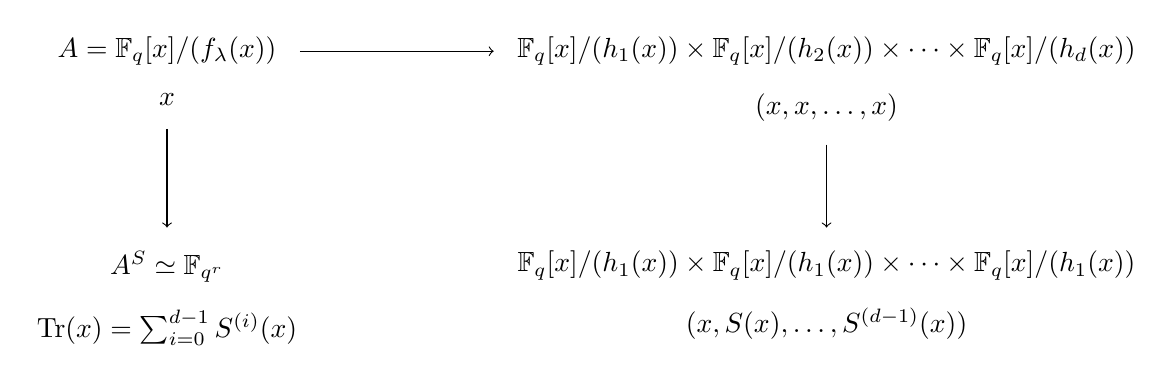
\begin{tikzpicture}
\node (A) {$A=\F_q[x]/(f_\lambda(x))$};
\node[below=.3em of A] (Ax) {$x$};
\node[right=8em of A] (CRT) {$\F_q[x]/(h_1(x)) \times \F_q[x]/(h_2(x)) \times \cdots \times \F_q[x]/(h_d(x))$};
\node[below=.3em of CRT] (CRTx) {$(x, x, \ldots, x)$};
\node[below=6em of A] (T) {$A^S \simeq \F_{q^r}$};
\node[below=.3em of T] (Tx) {$\mathrm{Tr}(x) = \sum_{i = 0}^{d-1} S^{(i)}(x)$};
\node[below=6em of CRT] (C) {$\F_q[x]/(h_1(x)) \times \F_q[x]/(h_1(x)) \times \cdots \times \F_q[x]/(h_1(x))$};
\node[below=.3em of C] (Cx) {$(x, S(x), \ldots, S^{(d-1)}(x))$};
\draw[->, shorten >= .5em, shorten <= .5em] (A) -- (CRT);
\draw[->, shorten >= .5em, shorten <= .5em] (Ax) -- (T);
\draw[->, shorten >= .5em, shorten <= .5em] (CRTx) -- (C);
\end{tikzpicture}
\end{center}

\begin{proposition}
\label{prop:xnormal}
If $x \in A$ is a normal element,
then $\eta_{\lambda,S}(P)$ is a normal element in $\F_{q^r}$
for any eigenpoint $P$ of $\lambda$.
\end{proposition}

\begin{proof}
Suppose that $x$ is normal in $A$, then so is its trace in $A^S$.
But taking the trace of $x$ in $A$ and going through the two isomorphisms
of the diagram is the same thing as computing the period in the
$d$ different representations of $\F_{q^r}$:
\[
x \mapsto \sum_{i=0}^{d-1} S^{(i)}(x) \mapsto
\left( \sum_{i=0}^{d-1} S^{(i)}(x) \pmod{h_1(x)}, \ldots,
\sum_{i=0}^{d-1} S^{(i)}(x) \pmod{h_d(x)} \right) \; .
\]
If a linear relation existed between $\eta_{\lambda,S}(P) \in \F_q[x(P)]$
and its Galois conjugates for any eigenpoint $P$ of $\lambda$,
it would be verified in the $d$ different representations of $\F_{q^r}$
and lift up to $A$ implying the same linear relation for
$\mathrm{Tr}(x)$ and its Galois conjugates.
Therefore, if $x$ is normal in $A$,
then $\eta_{\lambda,S}(P)$ is normal in $\F_q[x(P)]$.
\end{proof}

The converse is easily shown not to be true by experimentation.
There is also no relation between the normality of $x \in A$
and $x(P) \in \F_q[x(P)]$ for any eigenpoint $P$ of $\lambda$,
or between the normality of $x(P)$ and that of $\eta_{\lambda,S}(P)$.

Nonetheless, Proposition~\ref{prop:xnormal} shows that heuristically
$\eta_{\lambda,S}(P)$ has a high probability to be normal and therefore
to generate $\F_q[x(P)]$.
Indeed, supposing that $x \in A$ behaves as a random element
as far as normality is concerned, it has a rather high probability
of begin normal as the following lemma shows.
\begin{lemma}
\label{lemma:euleralgebra}
Let $A$ be a polynomially cyclic algebra of degree $dr$
over the finite field $\F_q$.
The number of normal elements in $A$ is the same as the
number of normal elements in $\F_{q^{dr}}$:
$\Phi_q(x^{dr}-1)$ where $\Phi_q$ is the Euler function
for polynomials.
\end{lemma}
\begin{proof}
There is at least one normal element in $A$~\cite[Theorem 4]{Mihailescu2010825}
(and it can be constructed from one in $\F_q$).
One such element $\alpha$ can be used to count the number of normal elements
as in the finite field case:
\begin{enumerate}
\item every element $a$ can be written using the normal basis
associated to $\alpha$: $a = \sum_{i=0}^{dr-1} a_i \nu^{(i)}(\alpha)$;
\item as the Galois group of $A$ is cyclic, the decomposition
of the Galois conjugates of $a$ is obtained by shifting the coefficients $a_i$;
\item the circulant matrix $M_a$ associated to the $a_i$'s is invertible
if and only if $a$ is a normal element;
\item the polynomial $\sum_{i=0}^{dr-1} a_i x^i$ in $\F_q[x] / (x^{dr}-1)$
is invertible if and only if $M_a$ is.
\end{enumerate}
Therefore normal elements in $A$ are in one-to-one correspondence
with units of $\F_q[x] / (x^{dr}-1)$.
\end{proof}

Another heuristic argument follows, supporting the fact that
elliptic periods should generate $\F_{q^r}$
at least when $q$ and $r$ are prime although it can be adapted to
a more general setting:
considering that $\eta_{\lambda, S}(P)$ behaves as a random
element of $\F_{q^r}$, the probability that it does not
generate $\F_{q^r}$, or equivalently that it lies in
the only strict subfield of $\F_{q^r}$ which is $\F_q$,
is $q^{1-r}$.
Therefore, counterexamples should be seeked for small values
of $q$ and $r$, but as stated in Appendix~\ref{app:ellprdsdata}
we found none so far.

To conclude this section, note that one might be tempted to
replace the trace above by any symmetric function of the
Galois conjugates of $x \in A$ such as the norm.
In the case of cyclotomic Gaussian periods,
replacing the trace by the norm either gives another root of unity
when the computation is trivial, or $1$ when it is not,
so such an operation has no sense.
But in the case of elliptic periods, there is no reason to expect such a
phenomenon.
However for most elementary symmetric functions, except for the trace,
couterexamples were found by small scale experiments.

\subsection{Elliptic variant of Rains' algorithm}

Rain's cyclotomic algorithm needs auxiliary extensions to accommodate
for sufficiently small subgroups $\mu_\ell$ of the unit group. By
replacing unit groups with torsion groups of elliptic curves, we gain
more freedom on the choice of the size of the group, thus we are able
to work with smaller fields.  

The algorithm is very similar to
Algorithm~\ref{algorithm:rains-cyclo}, and follows immediately from
the previous section. Given $k$, $K$ and $r$,
\begin{enumerate}
\item find a prime $\ell$, an elliptic curve $E$, and an eigenvalue
  $\lambda$ of the Frobenius endomorphism, satisfying the conditions
  of Theorem~\ref{theorem:ellperiods}, and such that
  $\order_\ell(\lambda)=r$;
\item take random points $P\in E(k)[\ell]$ and $P'\in E(K)[\ell]$ in
  the eigenspace of $\lambda$;
\item return the elliptic periods $\alpha_r := \eta_{\lambda}(P)$ and
  $\beta_r:= \eta_\lambda(P')$.
\end{enumerate}

Here we are faced with a difficulty: given $E$ and $\lambda$ it is
easy to pick a random point in $E[\ell]$, but it is potentially much
more expensive to compute a point in the eigenspace of $\lambda$. We
will circumvent the problem by forcing $E(\F_{q^r})[\ell]$ to be of
rank $1$, and to coincide exactly with the eigenspace of $\lambda$.
If we write $\mu = q/\lambda$ for the other eigenvalue of $\pi$, this
is easily ensured by further asking that $\order_\ell(\mu) \nmid r$.

We defer the discussion on the search for the elliptic curve $E$ to
Section~\ref{sec:selection}. Here we suppose we are already given
suitable parameters $\ell$, $E$ and $\lambda$, and analyze the last
two steps of the algorithm, summarized below.  We only give the
procedure for the smaller $k$, the procedure for the field $K$ being
identical.

\begin{algorithm}[Elliptic Rain's algorithm]
\label{algorithm:compell}
  \begin{algorithmic}[1]
    \REQUIRE A field extension $k/\F_q$ of degree $r$,
    an elliptic curve $E/\F_q$, its trace $t$, a prime $\ell$ not dividing $q$,
    an integer $\lambda$ such that:
    \begin{itemize}
    \item $X^2 - tX - q = (X-\lambda)(X-q/\lambda) \mod\ell$,
    \item $\order_\ell(\lambda)=r$, $\order_\ell(q/\lambda)\nmid r$,
    \item $(\Z/\ell\Z)^{\ast}/\Aut_{\F_q}(E) = \langle{\lambda}\rangle \times S$ for some $S$.
    \end{itemize}
    \ENSURE A generator of $k$ over $\F_q$, with a uniquely defined Galois orbit.
    \REPEAT
    \STATE Compute $P\leftarrow[\# E(k)/\ell]Q$ for a random $Q\in E(k)$;
    \UNTIL{$P\neq\mathcal{O}$;}
    \RETURN $\alpha_r\leftarrow\eta_\lambda(P)$.
  \end{algorithmic}
\end{algorithm}

\begin{proposition}
  Algorithm (\ref{algorithm:compell}) is correct. On input
  $r,q,E,t,\ell,\lambda$ it computes its output using
  $O(\MM(r)(r\log{q} + (\ell/r)\log{\ell})$ operations in $\F_q$, or
  $\tildO(r^2\log q)$ assuming $\ell\in o(r^2)$.
\end{proposition}
\begin{proof}
  By construction the point $P$ has $r$ distinct conjugates in
  $k$, and, since $r$ is odd, all have distinct abscissas,
  hence $x(P)$ generates $k$.  The correctness of the algorithm
  then follows immediately from Theorem~\ref{theorem:ellperiods} and
  the discussion above.

  From the knowledge of the trace $t$, we immediately determine the
  zeta function of $E$, and hence the cardinality $\# E(k)$, at
  no algebraic cost.

  To select the random point $Q\in E(k)$ we take a random
  element $x\in k$, then we verify that it is the abscissa of a
  point using a squareness test, at a costs of $O(r\MM(r)\log q)$
  operations. Then, using Montgomery's formulas for scalar
  multiplication~\cite{montgomery}, we can compute the points $P$ and
  $[\ell]P$ without the knowledge of the ordinate of $Q$, at a cost of
  $O(r\MM(r)\log q)$ operations. A valid point is obtained after
  $O(1)$ tries on average.

  The elliptic period in the final step requires $O(\ell/r)$ scalar
  multiplications by an integer less than $\ell$, for a total cost of
  $O((\MM(r)\ell\log\ell)/r)$.
\end{proof}


\section{Algorithm selection}
\label{sec:selection}

The algorithms presented in the previous sections have very similar
complexities, and no one stands out as absolute winner. The complexity
of all algorithms, besides the naive one, depends in a non-trivial way
on the parameters $q$ and $r$, and, for Rains' algorithms, on the
search for a parameter $\ell$ and an associated elliptic curve.

This section studies the complexity of the embedding description
problem from a global perspective. We give procedures to find
parameters for Rains' algorithms, criteria to choose the best among
the embedding algorithms, and asymptotic bounds on the embedding
description problem.


\subsection{Finding parameters for Rains' algorithms}

Given parameters $q$ and $r$, Rains' cyclotomic algorithm asks for a
\emph{small} parameter $\ell$ such that:
\begin{enumerate}
\item $(\Z/\ell\Z)^\ast = \langle q\rangle \times S$ for some $S$,
\item $\langle q \rangle = rs$ for some integer $s$.
\end{enumerate}

Since $r$ is a prime power, the second condition lets us take a prime
power for $\ell$ too. Indeed if
$\Z/\ell\Z\simeq\Z/\ell_1\Z\times\Z/\ell_2\Z$, then either
$q\bmod\ell_1$ or $q\bmod\ell_2$ has order a multiple of $r$.
Furthermore, if $\gcd(\ell,r)=1$, then we can take $\ell$ prime, since
higher powers would not help satisfy the conditions. On the other
hand, if $\gcd(\ell,r)\ne1$, then Kummer-type algorithms have better
complexity \todo{double-check this}, hence we shall take $\ell$ prime.

Given the above constraints, we can rewrite the conditions as:
\begin{enumerate}
\item $\ell = rsu + 1$ for some $s,u$ such that $\gcd(rs,u)=1$,
\item $\order_\ell(q) = rs$.
\end{enumerate}

\begin{remark}
  Rains remarked that, when $q=2$ and $r$ is a power of $2$ greater
  than $4$, no $\ell$ can satisfy these constraints because $2$ is a
  quadratic residue modulo any prime of the form $8u+1$. This case,
  however, is covered by the Artin-Schreier technique in
  Section~\ref{sec:artin-schreier-case}, we thus ignore it.
\end{remark}

In the elliptic algorithm we look for an integer $\ell$ and a curve
$E/\F_q$ that satisfy the preconditions of
Algorithm~\ref{algorithm:compell}, i.e., such that 
\begin{enumerate}
\item the Frobenius endomorphism $\pi$ satisfies a characteristic
  equation $(\pi-\lambda)(\pi-\mu) = 0 \mod \ell$,
\item $(\Z/\ell\Z)^\ast = \langle\lambda\rangle\times T$ for some $T$,
\item $\#\langle\lambda\rangle=r$, and
\item $\mu^r\ne1\mod\ell$.
\end{enumerate}

As before, we only need to look at prime $\ell$. For simplicity, we
also exclude the case where $r$ is a power of $2$, which is easily
dealt with Kummer-type algorithms. Because $\mu=q/\lambda$, the last
condition is equivalent to $q^r\ne1\bmod\ell$. Hence, we can restate
the conditions on $\ell$ as
\begin{enumerate}
\item $\ell = ru+1$ for some $u$ such that $\gcd(r,u)=1$,
\item $q^r\ne1\mod\ell$.
\end{enumerate}
Once $\ell$ is found, we compile a list of all integers of order $r$
in $(\Z/\ell\Z)^\ast$, and look for a curve of trace
$t=\lambda+q/\lambda\bmod\ell$ for any $\lambda$ in the list. Note,
however, that for there to be such a curve, $t$ must have a
representative in the interval $[-2\sqrt{q},2\sqrt{q}]$. In order to
have a good chance of finding such curves, we are going to set an even
more stringent bound $\ell\in o(\sqrt[4]{q})$.

We propose a procedure to simultaneously find parameters for the
cyclotomic and the elliptic case in
Algorithm~\ref{algorithm:selectell}. The procedure is given bounds on
the size of the parameters sought, and outputs all suitable parameters
within those bounds.

\begin{algorithm}
    [Parameter selection for Rains' algorithms]
    \label{algorithm:selectell}
    \begin{algorithmic}[1]
      \REQUIRE Integers $q$ and $r$, bounds $\bar{u}$, $\bar{s}$, and $\bar{e}$;
      \ENSURE $\mathcal{C}$ and $\mathcal{E}$, lists of parameters for the cyclotomic and elliptic algorithm resp.
      \STATE $\mathcal{C}\leftarrow\{\}$, $\mathcal{E}\leftarrow\{\}$;
      \FOR{$u=1$ to $\bar{u}$}
      \IF{\label{alg:selectell:prime}$\ell=ur+1$ is prime}
      \IF{\label{alg:selectell:order}$\order_\ell(q)=rs$ with $s\le\bar{s}$ and $\gcd(rs,u/s)=1$}
      \STATE Add $\ell$ to $\mathcal{C}$.
      \ENDIF
      \IF{\label{alg:selectell:ellorder}$\ell\le\bar{e}$ and $\gcd(u,r)=1$ and $q^r\ne1\bmod\ell$}
      \STATE Compute $\mathcal{T} \leftarrow \{\lambda + q/\lambda \bmod\ell \;|\; \order_\ell(\lambda)=r\}$;
      \REPEAT\label{alg:selectell:ellloop}
      \STATE\label{alg:selectell:ellcount} Take random $E/\F_q$ and compute its trace $t$;
      \UNTIL{$(t\bmod\ell)\in\mathcal{T}$}
      \STATE Add $(\ell,E,t)$ to $\mathcal{E}$.
      \ENDIF
      \ENDIF
      \ENDFOR
      \RETURN $\mathcal{C}$ and $\mathcal{E}$.
    \end{algorithmic}
\end{algorithm}

\begin{proposition}
  On input $q$, $r$, $\bar{u}$ and $\bar{e}$,
  Algorithm~\ref{algorithm:selectell} computes its output using
  $\tildO\left(\sqrt{r\bar{u}^3} + \bar{u}^2\log^6{q}\right)$ binary
  operations, assuming $\bar{e}\in o(\sqrt[4]{q})$.
\end{proposition}
\begin{proof}
  We only consider naive integer arithmetic, since it is unrealistic
  to apply embedding algorithms to very large sizes.

  In Step~\ref{alg:selectell:prime} we need to test for the primality
  of $\ell$, while Steps~\ref{alg:selectell:order}
  and~\ref{alg:selectell:ellorder} require the factorization of
  $\ell-1$. Both operations can be performed in
  $\tildO(\sqrt{r\bar{u}})$ operations using naive algorithms.

  In Step~\label{alg:selectell:ellcount} we need to count the number
  of points of an elliptic curve over $\F_q$. This can be done in
  $O\left(\log^6(q)\right)$ binary operations using the
  Schoof-Elkies-Atkin algorithm with naive integer
  arithmetic~\cite{schoof95,lercier+sirvent08}. Knowing the trace of a
  curve $E$ we immediately know the traces of its twists (see
  Appendix~\ref{app:elliptic-curves}).

  All other operations have negligible cost compared to these ones. We
  finally need to account for the two loops in the algorithm. The
  inner loop at Step~\ref{alg:selectell:ellloop} stops when a curve
  with $t\bmod\ell$ in $\mathcal{T}$ is found. The set $\mathcal{T}$
  has size $\euler(r)$, hence, assuming that traces are evenly
  distributed modulo $\ell$, we expect to find a suitable curve after
  $O(\ell/r)\subset O(\bar{u})$ tries. Although it is well known that
  traces are not evenly distributed modulo prime
  numbers~\cite{lenstra87}, it is shown
  in~\cite[Th.~1]{castryck+hubrechts13} that the probability that a
  random curve has trace congruent to a fixed $t\bmod\ell$ approaches
  $1/\ell$, as $\ell$ and $q$ go to infinity, subject to $\ell\in
  o(\sqrt[4]{q})$. Hence, we shall assume that $\bar{e}\in
  o(\sqrt[4]{q})$ for the complexity analysis to hold.

  The outer loop multiplies the whole complexity by $\bar{u}$, we
  conclude that the overall complexity is in
  $\tildO\left(\sqrt{r\bar{u}^3} + \bar{u}^2\log^6{q}\right)$.
\end{proof}


\subsection{Selecting the best algorithm}

A natural question arises: what bounds $\bar{u},\bar{s},\bar{e}$ must
be taken to ensure that the lists $\mathcal{C}$, $\mathcal{E}$ in
Algorithm~\ref{algorithm:selectell} are non-empty?

It is not easy to give a precise answer: already the condition in that
$\ell=ur+1$, in Step~\ref{alg:selectell:prime}, poses some
difficulties. Heuristically, we expect that about
$\bar{u}/\log(\bar{u}r)$ of those numbers are prime. However the best
lower bound on primes of the form $\ell=ur+1$, even under GRH, is
$\ell\in O(r^{2.4+\epsilon})$~\cite{heath1992zero}. Empirical data
show that the reality is much closer to the heuristic bound: in
Figure~\ref{fig:primes-arith-prog} we plot for all prime powers
$r<10^8$ the smallest $u$ such that $ur+1$ is prime. It appears that
$u$ is effectively bounded by $O(\log r)$ for any practical purpose.


\begin{figure}
  \centering
  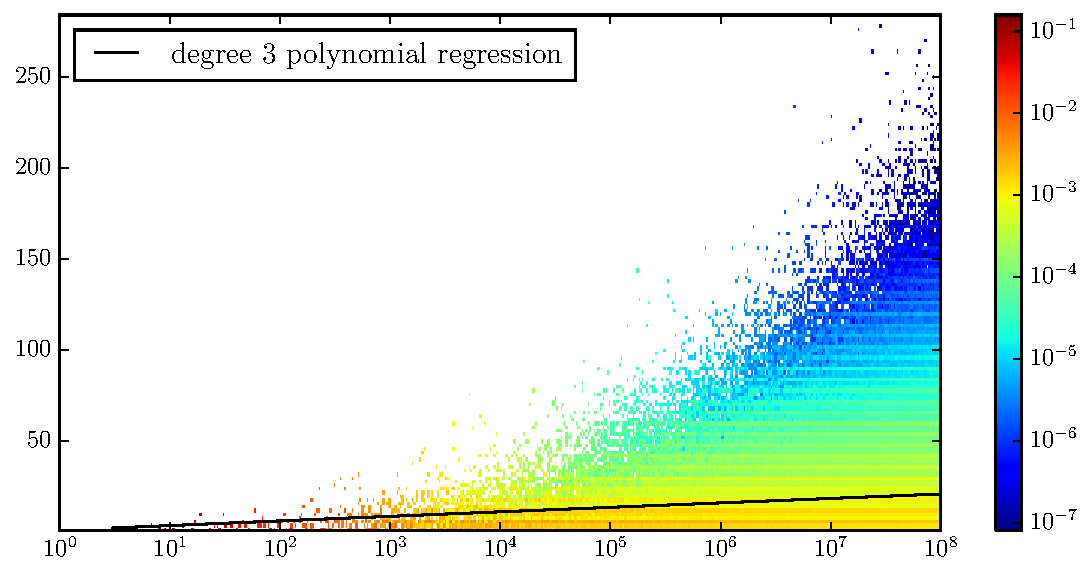
\includegraphics[width=\textwidth]{arith_prog}  
  \caption{Prime powers $r$ (abscissa) versus smallest integer $u$
    (ordinate) such that $ur+1$ is prime. Abscissa in logarithmic
    scale, density normalized by $\log(x)/x$ and colored in
    logarithmic scale.}
  \label{fig:primes-arith-prog}
\end{figure}

For the cyclotomic algorithm we also require that $\order_\ell(q)$ is
a multiple of $r$. Assuming that $q$ is uniformly
distributed\footnote{This assumption is obviously false for any fixed
  $q$, but it is a good enough approximation in practice.} in
$(\Z/\ell\Z)^\ast$, its order is exactly $\ell-1$ with probability
$(\ell-1)/\ell$, hence we can assume that asymptotically
$\order_\ell(q)\in O(\ell)=O(r\log r)$. Similar considerations can be
made for the elliptic algorithm, assuming that $\ell\in
o(\sqrt[4]{q})$.

Summarizing, if we take $\bar{u},\bar{s}\in O(\log r)$, we can expect
Algorithm~\ref{algorithm:selectell} to find suitable parameters for
the cyclotomic algorithm, leading to expected parameters $\ell\in
O(r\log r)$, and to an expected running time of $\tildO(\sqrt{r})$
binary operations and $\tildO(r^2\log q)$ operations in
$\F_q$. \todo{Shall we also consider the second variant of cyclotomic
  algorithm?} Similarly, if we also take $\bar{e}\in O(r\log r)$,
assuming that $r\log r\in o(\sqrt[4]{q})$, we can expect
Algorithm~\ref{algorithm:selectell} to find suitable parameters for
the elliptic algorithm, leading to an expected running time of
$\tildO(\sqrt{r}+(\log r)^2(\log q)^6)$ binary operations and
$\tildO(r^2\log q)$ operations in $\F_q$. \todo{Shall we extend the
  applicability of the elliptic algorithm by taking small extensions
  of the base field?}

Although the complexities of both algorithms look very similar, it
must not be neglected that the $\tildO$ notation in the cyclotomic
algorithm hides the cost of taking an auxiliary extension of degree
$O(\log^2r)$; whereas the elliptic algorithm, when it applies, does
not incur such overhead. The impact of the hidden terms in the
complexity can be extremely important, as we will show in the next
section. 

The same considerations also apply when comparing Rains' algorithms to
the other ones: the root-based and the Kummer-type algorithms perform
extremely well when the degree $s$ of the auxiliary extension is
small, but become much slower as this degree increases (recall that
asymptotically $s\in O(r)$ \todo{Make this more precise, if it is not
  done in the previous sections}).

In practice, it is hopeless to try and determine the appropriate
bounds for each algorithm from a purely theoretical point of view. The
best approach we can suggest, is to determine parameters at runtime,
and set bounds and thresholds experimentally. We summarize our
suggested approach in Algorithm~\ref{algorithm:selectalg}. 

\begin{algorithm}
  [Algorithm selection]
  \label{algorithm:selectalg}
  \begin{algorithmic}[1]
    \REQUIRE Integers $q$ and $r$, bounds $\bar{u}$, $\bar{s}$, and $\bar{e}$, etc.
    \STATE \todo{}
  \end{algorithmic}
\end{algorithm}

\todo{Talk about gluing prime powers.}


\section{Experimental Results}

To validate our results, we implemented the algorithms described in
the previous sections, and compared them to the implementation of
Allombert's algorithm available in Pari/GP~\cite{Pari}. The variants
of Allombert's algorithm described in Section~\ref{sec:fast-kummer}
were implemented in C on top of the Flint
library~\cite{hart2010flint}. Rains' cyclotomic and elliptic
algorithms were implemented in Sage~\cite{Sage} (which itself uses
Pari and Flint for representing finite fields), with critical code
rewritten in C/Cython (\todo{JP, do you want to give a better pointer
  to ellmul?}). Our code only handles $q$ prime and $m,n$ odd.

We ran tests for a wide range of primes $q$ between $5$ and
$2^{60}+3175$, and prime powers $r$ between $5$ and $1021$. All tests
were run on an Intel \todo{JP, what can you tell us?}. We report in
Figure~\ref{fig:bench} statistics only on the runs for
$2^{10}<q<2^{13}$; other ranges show very similar trends. The source
code and the full datasets can be downloaded at
\url{https://github.com/defeo/ffisom}.



\begin{figure}
  \newlength{\mywidth}
  \setlength{\mywidth}{8cm}
  \centering

  \begin{subfigure}{.48\textwidth}
    \includegraphics[width=\mywidth]{bench-allombert}
    \caption{Pari/GP and our own variants of Allombert's algorithm.
      Auxiliary extension degrees $s$ range between $1$ and $6$.}
    \label{fig:bench:allombert}
  \end{subfigure}
  \hfill
  \begin{subfigure}{.48\textwidth}
    \noindent
    \includegraphics[width=\mywidth]{bench-rains}
    \caption{Cyclotomic and elliptic variants of Rains' algorithm.
      Auxiliary extension degrees $s$ for cyclotomic Rains' range
      between $1$ and $8$.}
    \label{fig:bench:rains}
  \end{subfigure}
  
  \begin{subfigure}{.48\textwidth}
    \noindent
    \includegraphics[width=\mywidth]{bench-all}
    \caption{Comparison of Allombert's and Rains' algorithms at some
      fixed, small, auxiliary extension degrees $s$.}
    \label{fig:bench:all}
  \end{subfigure}
  \hfill
  \begin{subfigure}{.48\textwidth}
    \noindent
    \includegraphics[width=\mywidth]{bench-allombert-vs-ell}
    \caption{Ratio between running time of Allombert's algorithm and
      average running time of elliptic Rains' algorithm at same degree
      $r$.}
    \label{fig:bench:allombert-vs-ell}
  \end{subfigure}

  \caption{Benchmarks for Rains' and Allombert's algorithms. $q$ is a
    prime between $2^{10}$ and $2^{13}$, $r$ is an odd prime power varying
    between $5$ and $509$.  Lines represent a batch of runs with
    constant auxiliary degree $s$ ($s$ is $\order_r(q)$ for
    Allombert's algorithm, $\order_\ell(q)/r$ for Rains' algorithm),
    averaged over the abscissa. Dots represent individual runs.
    Plots~\subref{fig:bench:allombert},~\subref{fig:bench:rains}
    and~\subref{fig:bench:all} are in doubly logarithmic scale. Full
    dataset available at \url{https://github.com/defeo/ffisom}.}
  \label{fig:bench}
\end{figure}

In Figure~\ref{fig:bench:allombert} we compare the implementation of
Allombert's algorithm in Pari/GP with our own, specifically the
variant which is dubbed \emph{``case 2''} in
Section~\ref{sec:fast-kummer}. Each continuous line represents a batch
of runs of the cyclotomic variant with constant auxiliary degree
$s=\order_r(q)$, ranging from $1$ to $6$; runs with the same degree
$r$ are averaged together. In both implementations we observe a large
gap between $s=1$ and other values of $s$, due to the added cost of
computing in extension rings. While our variant performs better for
very small degree, it quickly catches and surpasses Pari in most
cases. However, our variant is considerably faster than Pari's when
the parameter $s$ gets larger, as we shall discuss in a few moments.

In Figure~\ref{fig:bench:rains} we compare the cyclotomic and elliptic
variants of Rains' algorithm. Each continuous line represents a batch
of runs of the cyclotomic variant with constant auxiliary degree
$s=\order_\ell(q)$, ranging from $1$ to $8$; runs with the same degree
$r$ are averaged together. Lines are clearly stacked on top of one
another according to their parameter $s$, only with occasional
crossings. We observe a very large gap between $s=1$ and larger $s$
($s=2$ is $8-16$ times slower). This is partly due to the fact that we
use generic Python code to construct auxiliary extensions, rather than
dedicated C; however a large gap is unavoidable, due to the added cost
of computing in extension fields. Dots represent individual runs of
the elliptic variant. We observe that on average it runs at a speed
which is intermediate between the cyclotomic variant with $s=2$ and
$s=3$. We wrote dedicated C code with optimized formulas for the
elliptic curve group operation, thus it seems difficult to improve the
gap between the elliptic and the cyclotomic variant. In conclusion the
cyclotomic variant only looks preferable to the elliptic one for very
small $s$, or when the elliptic variant does not apply.

To get a global view, we graph all algorithms in
Figure~\ref{fig:bench:all}. It appears that Allombert's algorithm
performs generally better than Rains' cyclotomic algorithm for small
auxiliary extension degree. Only when the $s$ parameter for
Allombert's algorithm reaches about $10$, it gets slower than Rains'
algorithm with $s=1$. The elliptic variant is even further up the
scale.

To more accurately determine the cross-points between the algorithms
we need to change picture. In Figure~\ref{fig:bench:allombert-vs-ell},
for every degree $r$ we compute the average running time of the
elliptic variant, then for each run of Allombert's algorithm (both in
Pari and in our version) we plot the ratio between its running time
and the average running time of the elliptic variant for the same
degree. We sort the ratios by increasing auxiliary extension degree
$s$ for Allombert's algorithm. It is then apparent that Pari's
implementation has a linear dependency in $s$, while our variant only
depends on it sub-linearly, as expected. This trend is even more
apparent with smaller primes $q$ and larger degrees $r$. The point
where both algorithms cross the elliptic variant of Rains' happens
around $s=100$. By postulating a constant ratio between Rains'
cyclotomic and elliptic variants, this graph can be used to determine
a cross-point for Allombert's \emph{versus} Rains' cyclotomic
algorithm too.

Obviously, these comparisons are only relevant to our own code and
test conditions. Other implementations and benchmarks will likely find
slightly different cross-points for the algorithms. Our goal here is
simply to show that all algorithms presented in this paper are
practical, that for each one there are specific parameters where it
performs best, and that our proposed variants constitute an
improvement over the state of the art.


%%%%%%%%%%%%%%%%%%%%%%%%%%%%%%%%%%
%%%%%%%%%%%%%%%%%%%%%%%%%%%%%%%%%%

\part{Embedding evaluation}
\label{part:eval}


\subsubsection{Linear algebra}

Once $\beta \in K$ has been computed as a polynomial in $Y$,
one can compute the powers
$\beta^i = \sum_{j=0}^{n-1} m_{i,j} Y^j$
for $i \in \{0, \ldots, n-1\}$ and build a matrix
$M = \{m_{i, j}\}_{0\leq i \leq m-1, 0 \leq j \leq n -1}$
representing $\phi$.
This is trivially done in $O(m)$ operations in $K$.
For $\gamma = \sum_{i = 0}^{m - 1} c_i X^i \in k$,
$\phi(\gamma)$ can then be computed by a
matrix-vector multiplication in $O(m n)$ operations in $\F_q$.

Together, the second and third questions are the inverse image problem.
They can be answered by first computing 
an LU or similar matrix decompostions of $M$
in $O((n (m)^{\omega - 1})$ operations in $\F_q$.
Answering the second and third questions together is then
an easy matter.

Note that if $m = n$, that is if $k$ and $K$ are
isomorphic, then the second question is trivial.
For the third one, the inverse
the inverse $M^{-1}$ of $M$ representing $\phi^{-1}$
can be deduced from an an LU or similar matrix decompostions of $M$.
For $\delta \in K$, $\phi^{-1}(\delta)$ can then be computed by a
matrix-vector multiplication in $O(m^2)$ in $\F_q$.

\subsubsection{Modular composition}

As an alternative to using linear algebra,
$\phi(\gamma)$ can be computed directly using modular composition
as $\beta(\gamma) \pmod{g}$ in $\CC(n)$ operations in $\F_q$.

The second question can be answered by performing a modular
exponentiation to check that $\gamma^{q^{m}} = 1$
naively in $O(m \log q)$ operations in $K$
or in $O(\log q)$ operations in $K$ plus
$O(\log m) \CC(n)$ operations in $\F_q$ using modular composition.

The second and third questions can be answered using
dual bases and power projection/transposed modular composition
to express $\delta \in K$ as a polynomial in $\beta$ in
$\CC(n)$ operations in $\F_q$.


%%%%%%%%%%%%%%%%%%%%%%%%%%%%%%%%%%

\section{Algorithms specific to normal bases}

In one of their article \cite{}, Kaltofen and Shoup proposed a subquadratic
implementation of the Black Box Berkelamp Algorithm, a probalistic algorithm to
factor a monic square free polynomial over finite fields. They mention that
an implementation of an automorphism projection algorithm can be used to solve 
the conversion to a normal basis coordinates problem. For a complete description
of the factorization algorithm, we redirect the reader to the section 3 of 
\cite{}. We focus on describing their implementation to help solve our problem.

Given an irreducible polynomial $f\in\F_q[X]$ of degree $n$, a normal element 
$\eta$ and an element $\gamma\in\F_q[X]/f(X)$, we wish to compute $c_0,\dots,
c_{n-1}\in\F_q$ such that :
\begin{equation}
\label{eq:eqnorm}
\gamma=c_0\eta+\dots+c_{n-1}\eta^{q^{n-1}}.
\end{equation}
Let $u$ be a projection map from $\F_{q^n}$ to $\F_q$. To solve this problem, 
We apply $n-1$ times the $q$-th power to (\ref{eq:eqnorm}), and apply $u$ to 
to each equations to obtain the following system in $\F_q$
\begin{equation}
\label{eq:systemnormal}
u(\gamma^{q^j})=\sum_{i=0}^{n-1}{c_iu(\eta^{q^{i+j}})}\qquad(0\leq j<n).
\end{equation}
We introduce the $n\times n$ matrix $Q$ used in the Berlekamp algorithm, its
$q_{i,j}$'s are the coefficients of
$X^{iq}=q_{i,n-1}X^{n-1}+q_{i,n-2}X^{n-1}+\dots+q_{i,0}\bmod f(X)$. It 
is the representation of the $q$-th power map on $\F_q[X]/f(X)$.
We can then rewrite (\ref{eq:systemnormal}) as
\begin{equation}
\label{eq:linalgnormal}
\vec{u}^\top Q^j\vec{\gamma}= \vec{c}\,(\vec{u}^\top Q^{i+j}\vec{\eta})_{i,j}
\qquad(0\leq j<n, 0\leq i<n),
\end{equation}
where $\vec{c}^\top=(c_0,c_1,\dots,c_{n-1})$, $\vec{\gamma}$ and $\vec{\eta}$
are the vectors containing the coordinates of $\gamma$ and $\eta$, respectively, 
in respect with the power basis.

The algorithm we are interested in focuses on computing the elements of the form 
$\vec{u}^\top Q^j\vec{\gamma}$, \emph{i.e.} solves the automorphism projection 
problem. To optimize the computation, the algorithm is be paramterized by a
$0\leq\beta\leq1$. We split the computation in several parts, set 
$t=\lceil{n^\beta}\rceil$ and $m=\lceil{k/t}\rceil$, where $k=o(n)$, the 
elements we want to compute are
\begin{equation}
\label{eq:normalsplit}
(\vec{u}^\top Q^{tj})\cdot(Q^l\vec{\gamma})\qquad(0\leq j<m, 0\leq l <t).
\end{equation}
In our case, we fix $k=n$.

\begin{algorithm}
  [Automorphism Projection]
  \label{algorithm:autoproj}
  \begin{algorithmic}[1]
    \REQUIRE $u$ defined as above, $\gamma$ an element of $\F_q[X]/f(X)$ and 
$0\leq\beta\leq1$.
    \ENSURE $(\vec{u}^\top Q^i\vec{\gamma})$ for $0\leq i<k$.
    \STATE $b_l\leftarrow Q^l\vec{\gamma}$ for $0\leq l<t$.
    \STATE Compute $X^{q^t}\bmod f(X)$.
    \STATE $a_j\leftarrow\vec{u}^\top Q^{tj}$ for $0\leq j<m$.
    \RETURN $(a_j.b_l)_{l+tj=i}$ for $0\leq i<n$.
  \end{algorithmic}
\end{algorithm}

The first step is done using a simple square and multiply algorithm, since
the left mulitplication by $Q$ is equivalent to raising to $q$. For the second 
step we use the Algorithm 5.2 from \cite{} of von Zur Gathen and Shoup. It only 
remains to compute $m-1$ transposed modular composition to carry out the right 
multiplications by $Q^t$. We have the following result :

\begin{theorem}
There exist probabilistic algorithms that can solve the above problem in 
\begin{equation}
O(n^{(\omega+1)/2+(1-\beta)(\omega-1)/2+o(1)}+n^{1+\beta+o(1)}\log{q})
\end{equation}
arithmetic operations in $\F_q$ for any $\beta$ with $0\leq\beta\leq1$.
Furthermore, for a specific choice of parameters, the cost of operations is
exactly $O(n^{1.815})\log{q}$.
\end{theorem}

\begin{proof}
See~\cite[Theorem 6]{}
\end{proof}

%%%%%%%%%%%%%%%%%%%%%%%%%%%%%%%%%%

\section{Monomial-dual bases pairs}

%%%%%%%%%%%%%%%%%%%%%%%%%%%%%%%%%%

\section{Experimental results}

%%%%%%%%%%%%%%%%%%%%%%%%%%%%%%%%%% 

\section{Conclusion}

%%%%%%%%%%%%%%%%%%%%%%%%%%%%%%%%%%
%%%%%%%%%%%%%%%%%%%%%%%%%%%%%%%%%%

\appendix
\part*{Appendices}
\addcontentsline{toc}{part}{Appendices}

%%%%%%%%%%%%%%%%%%%%%%%%%%%%%%%%%%

\section{Elliptic curves}
\label{app:elliptic-curves}


% Another subtlety arises in comparison with multiplicative groups:
% elliptic curves always come with non trivial automorphisms. We recall
% that the size of the \emph{group of rational automorphisms} of a curve
% $E/\F_q$ is one of the following:
% \begin{itemize}
% \item $\#\Aut_{\F_q}(E) = 12$ if $j(E)=0$ and $q=0\mod 9$ \todo{is this correct? useful?},
% \item $\#\Aut_{\F_q}(E) = 6$ if $j(E)=0$ and $q=1\mod 3$,
% \item $\#\Aut_{\F_q}(E) = 4$ if $j(E)=1728$ and $q=1\mod 4$,
% \item $\#\Aut_{\F_q}(E) = 2$ otherwise.
% \end{itemize}


Recall that two elliptic curves $E$ and $E'$ over a field $k$ are said
to be \emph{isomorphic} if there exists a linear change of variables
with coefficients in $k$ sending one onto the other. If $E$ and $E'$
are isomorphic over $\bar{k}$, but not over $k$, they are said to be
\emph{twists} of each other. A twist is said to be quadratic
(resp. cubic, quartic, sextic), if $E$ and $E'$ become isomorphic over
a quadratic (resp. cubic, quartic, sextic) extension of $k$. Most
elliptic curves only have quadratic twists; elliptic curves with
$j=0,1728$ may have cubic, quartic and sextic twists. See~\cite{Sil}.

We now give a proposition relating the number of points of an elliptic
curve over a finite field with the number of points of its twists.  In
the case of quadratic twists, this proposition simply states that $E$
and $E'$ have opposite trace, a well known fact.

\begin{proposition}
  \label{proposition:twisttrace}
  Let $E$ be an ordinary elliptic curve defined over a finite field
  $\F_q$ of characteristic $p\ne2$, and denote by $t$ the trace of its
  Frobenius endomorphism.

  Let $u\in\bar{\F}_q$, define a curve $E^u$ and an isomorphism
  $\upsilon$ of elliptic curves by
  \begin{equation*}
    \begin{aligned}
      \upsilon : E &\to E^u,\\
      (x,y) &\mapsto (u^2x,u^3y).
    \end{aligned}
  \end{equation*}
  If $E^u$ is defined over $\F_q$, then $u^{q-1}$ is an element of
  $\F_p$ of multiplicative order $n\in\{1,2,3,4,6\}$.

  Let $t_u$ be the trace of the Frobenius endomorphism of $E^u$, then
  $t_u^n=t^n \bmod q$, and $t_u=u^{q-1}t\bmod p$. This is enough to
  uniquely determine $t_u$ given $t$.
\end{proposition}
\begin{proof}
  Observe that if $E^u$ is a quadratic (resp. cubic, quartic, sextic)
  twist of $E$, then $u^{q-1}$ has multiplicative order $2$
  (resp. $3,4,6$). Furthermore, since $E$ is ordinary, $2$
  (resp. $3,4,6$) divides $p-1$, hence $u^{q-1}$ is in the prime field
  $\F_p$, and it defines a curve automorphism
  \begin{equation*}
    \upsilon^{q-1}:(x,y)\mapsto(u^{2q-2}x,u^{3q-3}y).
  \end{equation*}
  Any twist arises this way (see~\cite{Sil}).

  Denote by $\pi$ and $\pi_u$ the frobenius endomorphisms of $E$
  and $E^u$ respectively. They satisfy the equations
  \begin{equation}
    \label{eq:frob-char-twist}
    \pi^2 - [t]\pi + [q] = 0, \qquad \pi_u^2 - [t_u]\pi_u + [q] = 0,
  \end{equation}
  where $[m]$ denotes multiplication by $m$ on the elliptic curves. By
  straightforward calculation, we also verify that they satisfy the
  commutative diagram
  \begin{equation*}
    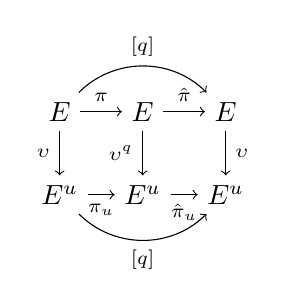
\begin{tikzpicture}[node distance=3em]
      \node(E){$E$};
      \node[right of=E](E2){$E$};
      \node[right of=E2](E3){$E$};
      \node[below of=E](Eu){$E^u$};
      \node[right of=Eu](Eu2){$E^u$};
      \node[right of=Eu2](Eu3){$E^u$};

      \draw[->,auto,font=\scriptsize]
      (E) edge node[swap]{$\upsilon$} (Eu)
          edge node{$\pi$} (E2)
          edge[bend left=45] node{$[q]$} (E3)
      (Eu) edge node[swap]{$\pi_u$} (Eu2)
           edge[bend right=45] node[swap]{$[q]$} (Eu3)
      (E2) edge node[swap]{$\upsilon^q$} (Eu2)
           edge node{$\hat\pi$} (E3)
      (Eu2) edge node[swap]{$\hat\pi_u$} (Eu3)
      (E3) edge node{$\upsilon$} (Eu3);
    \end{tikzpicture}
  \end{equation*}
  where we denote by $\upsilon^q$ the isomorphism
  $(x,y)\mapsto(u^{2q}x,u^{3q}y)$, and by $\hat\pi,\hat\pi_u$ the dual isogenies
  to $\pi,\pi_u$.

  Now we restrict the maps above to the $q$-torsion subgroups of $E$
  and $E^u$. Since the curves are ordinary, these subgroups are cyclic
  of order $q$, and the maps act as scalar multiplication on the
  points. In particular, we deduce from Eq.~\eqref{eq:frob-char-twist} that 
  \begin{equation*}
    \pi = [t \bmod q], \qquad \pi_u = [t_u \bmod q].
  \end{equation*}
  Hence, from the diagram we obtain
  \begin{equation*}
    [t] = \upsilon^{-q}\circ[t_u]\circ\upsilon \mod q.
  \end{equation*}

  Notice that $\upsilon^{-q}$ can be decomposed as
  $\upsilon^{-1}\circ\upsilon^{1-q}$, where $\upsilon^{1-q}$ is an
  automorphism of $E^u$ by hypothesis. $\upsilon^{1-q}$ also acts on
  the $q$-torsion points as a scalar in $\Z/q\Z$, that we shall denote
  by $U$. It is evident that the multiplicative order of $U$ in $\Z/q\Z$
  is the same as that of $u^{1-q}$ in $\F_p$. Then
  \begin{equation*}
    [t] = \upsilon^{-1}\circ[Ut_u]\circ\upsilon\mod q.
  \end{equation*}
  But $\upsilon$ is an isomorphism, thus it commutes with scalar
  multiplication, and we conclude that $t=Ut_u\bmod q$.

  If $u^{1-q}=\pm1$, we are done. When the order of $u^{1-q}$ is $3,4$
  or $6$, we still have to determine which of the cubic, fourth, sixth
  roots of unity in $\Z/q\Z$ corresponds to $U$.

  Using the diagram above, we decompose
  Eq.~\eqref{eq:frob-char-twist} as
  \begin{equation*}
    \hat\pi\circ\pi = [t]\pi - \pi^2,
  \end{equation*}
  and similarly for $E^u$. Hence, from the diagram again,
  \begin{equation}
    \label{eq:twisttrace:modp}
    [t] - \pi = \hat\pi = \upsilon^{-1}\circ\hat\pi_u\circ\upsilon^q 
    =  \upsilon^{-1}\circ([t_u] - \pi_u)\circ\upsilon^q.
  \end{equation}
  Let now $\omega$ be the invariant differential of $E$, we apply the
  pullback of Eq.~\eqref{eq:twisttrace:modp} to $\omega$. On the
  left-hand side we have
  \begin{equation}
    \label{eq:twisttrace:modp-lhs}
    ([t]-\pi)^\ast\omega = t\omega\in\Omega_E
  \end{equation}
  because $\pi$ is inserparable (see \cite[\S~5]{Sil}). On the
  right-hand side, if we let $\omega_u$ be the invariant differential
  of $E^u$, we have $(\upsilon^{-1})^\ast\omega=u\omega_u$, and
  $(\upsilon^q)^\ast\omega_u=\omega/u^q$, hence
  \begin{equation}
    \label{eq:twisttrace:modp-rhs}
    (\upsilon^{-1}\circ([t_u] - \pi_u)\circ\upsilon^q)^\ast\omega =
    u(([t_u] - \pi_u)\circ\upsilon^q)^\ast\omega_u =
    ut_u(\upsilon^q)^\ast\omega_u = u^{1-q}t_u\omega.
  \end{equation}
  Comparing Eqs.~\eqref{eq:twisttrace:modp-lhs}
  and~\eqref{eq:twisttrace:modp-rhs}, we conclude that $t = u^{1-q}t_u
  \bmod p$. Given that $\lvert t_u\rvert\le2\sqrt{q}$, we have uniquely determined $t_u$, and proven the theorem.
\end{proof}

\todo{Give a similar proposition for supersingular curves (see, e.g.,
  Menezes-Okamoto-Vanstone)}

\section{Elliptic periods and polynomial bases}
\label{app:ellprdsdata}

As discussed in Section~\ref{sec:ellperiods}, if counterexamples to
Conjecture~\ref{conj:ellperiods} are to be found, they should be seeked
for small values of $q$ and $r$ as the probability that a random element
does not generate $\F{q^r}$ is expected to decrease as $q^{-r}$.

There is variety of ways to check Conjecture~\ref{conj:ellperiods}:
\begin{itemize}
\item in general, compute a point of $l$-torsion defined
over $\F{q^r}$, the associated elliptic period and its minimal polynomial.
\item when $q$ and $r$ are prime (and elements of $\F{q^r}$ are represented
as polynomials of degree less than $r$ over $\F{q}$), it is enough to
check whether the elliptic period is a scalar (that is a constant polynomial)
or not.
\end{itemize}

It is also possible to avoid the computation of an actual $l$-torsion point
and of minimal polynomials.
For example, let $r$ be a prime such that $l = 4*r+1$ is prime
and suppose that $l$ is an Elkies prime for $E$:
the $l$-division polynomial $f_l$ of $E$ has two factors
$f_\lambda$ and $h_\lambda$ of degree $r$ over $\F{q}$.
The elliptic period is defined as $x(P) + x([i] P)$ for some
$i \in \left(Z / l \Z\right)^*$ such that $i^2 \equiv -1 \pmod{l}$
and any $P \in E(\F{q^r}[l]$
and the mapping $x + m_i(x)$ sends the roots of $f_\lambda$
and the roots of $h_\lambda$ onto the ellptic periods.
If we suppose that the period is not generating $\F{q}$ which implies that
$\Res_x(f_\lambda(x),y-x-m_i(x)) = \Res_x(h_\lambda(x),y-x-m_i(x))$
splits over $\F{q}$,
then by Galois invariance $x + m_i(x) \equiv t \pmod{f_\lambda}$
for a constant $t \in \F{q}$,
and since the periods do not depend on the initial choice of $f_\lambda$
or $h_\lambda$,
we conclude that $m_i(x) \equiv (t-x) \pmod{f_\lambda h_\lambda}$.
Hence, we can just compute $x + m_i(x) \pmod{f_\lambda h_\lambda}$
and see if it is a constant.
The dominating step in this approach is the factorization of $f_l$.
For large values of $q$ it could be replaced by using modular polynomials
and isogeny computations à la SEA, but the chances of finding counterexamples
are higher for small $q$'s.

Finally, remark that we can apply the above approach to elliptic curves
defined over the rationals and known to have rational $l$-torsion
over an extension of degree $r$.
One looks a prime number $q$
(outside primes of bad reduction or
with reduction giving more than a couple of automorphisms)
such that $q$ divides the content of $x + m_i(x)$.

One such curve is curve~\texttt{147b1} in Cremona's table~\cite{} which is
defined over $\Q$ and has $13$-torsion in a cubic extension.
Actually, for $l=13$ and $r=3$, all such curves belong to a parametrized family
exhibited by from Sutherland et al.~\cite{} with $j$-invariant:
\[
j(t)=\frac{\left(t^4-t^3+5 t^2 + t + 1\right) \left(t^8 - 5 t^7 + 7 t^6 - 5 t^5 + 5 t^3 + 7 t^2 + 5 t + 1\right)^3}{t^{13} \left(t^2 -3 t - 1\right)} \enspace .
\]

\todo{datadatadata}


%%%%%%%%%%%%%%%%%%%%%%%%%%%%%%%%%%
%%%%%%%%%%%%%%%%%%%%%%%%%%%%%%%%%%

\bibliographystyle{plain}
\bibliography{defeo}

\end{document}


% Local Variables:
% ispell-local-dictionary:"american"
% End:

%  LocalWords:  isomorphism cyclotomic coprime subfield Frobenius
%  LocalWords:  endomorphism eigenspace Allombert's
